\documentclass[a4paper,10pt]{article}
\usepackage[utf8]{inputenc}
\usepackage[nottoc,numbib]{tocbibind} % makes the BibTeX references section appear in the table of contents
\usepackage[inline]{enumitem}
\usepackage{amssymb}
\usepackage{amsfonts}
\usepackage{amsmath}
\usepackage{amsthm}
\usepackage[dvipsnames]{xcolor}
\usepackage{caption}
\usepackage{subcaption}
\usepackage{graphicx}
\usepackage{mathtools}
\usepackage{mathrsfs}
\usepackage{framed}
\usepackage{varioref}
\usepackage{adjustbox}
\usepackage{tablefootnote}
\usepackage{makecell}
% eventually make left/right margins equal
\usepackage[top=1in,bottom=1in,left=1.5in,right=1in]{geometry}
\usepackage{dsfont}

\usepackage{ulem}
\normalem


\usepackage[textwidth=0.7in]{todonotes}

\usepackage[hidelinks]{hyperref} %this needs to be loaded last!

% for 3D pictures
\usepackage{tikz}
\usepackage{tikz-3dplot}
\usetikzlibrary{perspective}

% for arrow/commutative diagrams
\usepackage{tikz-cd}

%prevent math mode statements from being broken up across lines
\relpenalty=9999
\binoppenalty=9999

%claim environment
\newenvironment{claim}[1]{\par\noindent\underline{Claim:}\space#1}{}

%leftbar
\renewenvironment{leftbar}[1][\hsize]
{%
    \def\FrameCommand
    {%
        {\vrule width 3pt}%
        \hspace{0pt}%must no space.
        \fboxsep=\FrameSep\colorbox{white}%
    }%
    \MakeFramed{\hsize#1\advance\hsize-\width\FrameRestore}%
}
{\endMakeFramed}

% fix footnote spacing
\let\oldfootnote\footnote
\renewcommand{\footnote}{\unskip\oldfootnote}
\newcommand{\olootodo}[1]{{\color{blue} #1}}
\newcommand{\ot}[1]{{\color{blue} #1}}
%numbering and style of theorems
\theoremstyle{plain}
\newtheorem{Theorem}{Theorem}
\newtheorem{Proposition}[Theorem]{Proposition}
\newtheorem{Corollary}[Theorem]{Corollary}
\newtheorem{Lemma}[Theorem]{Lemma}
\newtheorem{Question}[Theorem]{Question}
\newtheorem{Conjecture}[Theorem]{Conjecture}
\newtheorem{Assumption}[Theorem]{Assumption}
\newtheorem{Algorithm}[Theorem]{Algorithm}

\theoremstyle{definition}
\newtheorem{Definition}[Theorem]{Definition}
\newtheorem{Property}[Theorem]{Property}
\newtheorem{Notation}[Theorem]{Notation}
\newtheorem{Condition}[Theorem]{Condition}
\newtheorem{Example}[Theorem]{Example}
\newtheorem{Exercise}[Theorem]{Exercise}
\newtheorem{Introduction}[Theorem]{Introduction}
\newtheorem{Remark}[Theorem]{Remark}
\newtheorem*{Remark*}{Remark}

\theoremstyle{remark}

\newtheorem{case}{Case}[Theorem]

% make proofs use filled in black square instead of empty square
\renewcommand{\qedsymbol}{$\blacksquare$}
%\renewcommand\proof{\noindent\textit{\textbf{Proof. }}}
\newcommand{\modo}[3]{#1 \equiv #2 \pmod{#3}}
\newcommand{\nmodo}[3]{#1 \not\equiv #2 \pmod{#3}}
\newcommand{\R}{\mathbb{R}}
\newcommand{\Q}{\mathbb{Q}}
\newcommand{\N}{\mathbb{N}}
\newcommand{\Z}{\mathbb{Z}}
\newcommand{\Zpos}{\mathbb{Z}_{\geq 0}}
\renewcommand{\vec}[1]{\mathbf{#1}}
\newcommand{\dist}{\text{dist}}
\newcommand{\F}{\mathbb{F}}
\newcommand{\C}{\mathbb{C}}
\newcommand{\lin}{\text{lin}}
\newcommand{\cl}{\text{cl}}
\newcommand\norm[1]{\left\lVert#1\right\rVert}
\newcommand{\ONE}{\mathds{1}}
\newcommand{\generatedby}[1]{\left\langle#1\right\rangle}
\newcommand{\id}{\text{id}}
\DeclareMathOperator{\sgn}{sgn}
\newcommand\abs[1]{\left|#1\right|}
\newcommand\Gl{\text{GL}}
\DeclareMathOperator{\pam}{pam}
\DeclareMathOperator{\Ent}{Ent}
%lifted point array
\newcommand{\lpa}[1]{\Sigma({#1})}

\title{Icosahedral Virus Transitions: Computational Techniques \\ \large Kalamazoo College Senior Integrated Project}
\author{Xavier Silva \\ \small Advisors: Dr. Stephen Oloo and Dr. Dave Wilson}

\begin{document}

\maketitle

\tableofcontents

\newpage

\section{Abstract}

Icosahedral viruses have the symmetries of an icosahedron, which involves 2-fold, 3-fold, and 5-fold rotational symmetries.
We can characterize these virus capsids with finite sets of points (called a point array) which we realize in 6D (not just 3D) for the purpose of crystallography: our 6D point arrays naturally fit inside 6D icosahedral lattices. There are \(55\) standard point arrays (called \emph{one-base}) from which we build all the others.
We model virus maturation by 6D linear transformations (transitions) of point arrays that preserve some or all of icosahedral symmetry.
To find these transitions (preserving either the full icosahedral group symmetry or one of its maximal subgroups \(A_4, D_{10}, \text{ or } D_6\)) we solve matrix equations of the form \(TB_0 = B_1\) for \(T\), where \(T\), the transition matrix, is a \(6\times6\) matrix that depends on either 2, 4, 6, or 8 real variables and the matrices \(B_0\) and \(B_1\) are representations of the point arrays.
We employ parallel computation techniques to efficiently find transitions between these point arrays.
We are able to reproduce previously discovered transitions for the Cowpea Chlorotic Mottle Virus that preserve \(D_6\) symmetry, and we create a comprehensive list of what symmetries can be preserved between any possible combination of the \(55\) standard point arrays.

\section{Introduction}
Icosahedral viruses have the symmetries of an icosahedron, which involves 2-fold, 3-fold, and 5-fold rotational symmetries.
We can approximate these virus capsids with finite sets of points (called a point array) which we realize in 6D (not just 3D) for the purpose of crystallography: our 6D point arrays naturally fit inside 6D icosahedral Bravais lattices. 
There are \(55\) standard point arrays (called \emph{one-base}) from which we build all the others.
\footnote{
	See section \ref{section:all-one-base-point-arrays} for the list of all 55 one-base point arrays.
}
We model virus maturation by 6D linear transformations (transitions) of point arrays that preserve some or all of icosahedral symmetry.
% icosahedron shape
\tdplotsetmaincoords{60}{45}
\begin{figure}[h]
\centering
\begin{tikzpicture}[tdplot_main_coords]
	
	% Icosahedron vertices
	% phi = 1.61803
	\coordinate (A) at (0, 1, 1.61803);
	\coordinate (B) at (0, 1, -1.61803);
	\coordinate (C) at (0, -1, 1.61803);
	\coordinate (D) at (0, -1, -1.61803);
	
	\coordinate (E) at (1, 1.61803, 0);
	\coordinate (F) at (1, -1.61803, 0);
	\coordinate (G) at (-1, 1.61803, 0);
	\coordinate (H) at (-1, -1.61803, 0);
	
	\coordinate (I) at (1.61803, 0, 1);
	\coordinate (J) at (1.61803, 0, -1);
	\coordinate (K) at (-1.61803, 0, 1);
	\coordinate (L) at (-1.61803, 0, -1);
	
	% Draw Icosahedron edges
	\draw[dashed] (A) -- (C);
	\draw (A) -- (E);
	\draw (A) -- (G);
	\draw[dashed] (A) -- (I);
	\draw (A) -- (K);
	
	\draw (B) -- (D);
	\draw (B) -- (E);
	\draw (B) -- (G);
	\draw (B) -- (J);
	\draw (B) -- (L);
	
%	\draw (C) -- (A);
	\draw[dashed] (C) -- (F);
	\draw[dashed](C) -- (H);
	\draw[dashed] (C) -- (I);
	\draw[dashed] (C) -- (K);
	
%	\draw (D) -- (B);
	\draw[dashed] (D) -- (F);
	\draw (D) -- (H);
	\draw (D) -- (J);
	\draw (D) -- (L);
	
%	\draw (E) -- (A);
%	\draw (E) -- (B);
	\draw (E) -- (G);
	\draw[dashed] (E) -- (I);
	\draw (E) -- (J);
	
%	\draw (F) -- (C);
%	\draw (F) -- (D);
	\draw[dashed] (F) -- (H);
	\draw[dashed] (F) -- (I);
	\draw[dashed] (F) -- (J);
	
%	\draw(G) -- (A);
%	\draw(G) -- (B);
%	\draw(G) -- (E);
	\draw(G) -- (K);
	\draw(G) -- (L);
	
%	\draw (H) -- (C);
%	\draw (H) -- (D);
%	\draw (H) -- (F);
	\draw (H) -- (K);
	\draw (H) -- (L);
	
	% I goes to A, C, E, F
	\draw[dashed] (I) -- (J);
	
	% J is already covered
	
	\draw (K) -- (L);
	
	% Draw Icosahedron vertices
	\foreach \vertex in {A, B, C, D, E, F, G, H, I, J, K, L}
	\fill (\vertex) circle (2pt);
	
\end{tikzpicture}
\caption{The icosahedron.}
\label{fig:icosahedron}
\end{figure}

\noindent The symmetry group of the icosahedron is defined abstractly as follows.
\begin{Definition}[Icosahedral Group]
	The icosahedral group, which we denote by \(\mathcal{I}\), is the 60-element group given by the presentation \[\mathcal{I} := \generatedby{a, b | a^2 = b^3 = (ab)^5 = 1}.\]
\end{Definition}
\noindent We will work with the explicit realization of the icosahedral group given by the following 6D representation.
\[a = \begin{bmatrix}
	-1 & 0  & 0 & 0 & 0 & 0 \\
	0  & -1 & 0 & 0 & 0 & 0 \\
	0  & 0  & 0 & 0 & 1 & 0 \\
	0  & 0  & 0 & 0 & 0 & 1 \\
	0  & 0  & 1 & 0 & 0 & 0 \\
	0  & 0  & 0 & 1 & 0 & 0
\end{bmatrix} \quad b = \begin{bmatrix}
	0 & -1 & 0  & 0 & 0 & 0 \\
	0 & 0  & -1 & 0 & 0 & 0 \\
	1 & 0  & 0  & 0 & 0 & 0 \\
	0 & 0  & 0  & 0 & 0 & 1 \\
	0 & 0  & 0  & 1 & 0 & 0 \\
	0 & 0  & 0  & 0 & 1 & 0
\end{bmatrix}.\]
The matrix \( a \) is rotation along a 2-fold symmetry axis, \( b \) is rotation along a 3-fold symmetry axis, and the product \( ab \) represents a 5-fold symmetry.

The icosahedral group has 3 maxmial subgroups, which we call \( A_4 \), \( D_{10} \), and \( D_6 \).
\footnote{Like the icosahedral group, these subgroups are also each generated by two \( 6 \times 6 \) matrices.} 
These are subsets of the symmetries of an icosahedron, corresponding to the symmetries of the tetrahedron, pentagonal prism, and triangular prism respectively as shown in figure \vref{fig:maximal_subgroups}.
% maximal subgroup figures
\tdplotsetmaincoords{82}{20}
\begin{figure}[h]
	\captionsetup{width=0.75\textwidth}
	\centering
	% A4
	\begin{tikzpicture}[scale=0.5, tdplot_main_coords,
		declare function={b=5;h=4.33;l=15;}]
		\draw[fill=gray,fill opacity=0.3] (b/2,-l/2,0)  -- (0,-l/2,h) -- (-b/2,-l/2,0) -- cycle;
		% \draw (b/2,-l/2,0) -- (0, l-20, h/3);
		% \draw (0,-l/2,h) -- (0, l-20, h/3);
		% \draw (-b/2,-l/2,0) -- (0, l-20, h/3);
		\draw (b/2,-l/2,0) -- (0, 0, h/3);
		\draw (0,-l/2,h) -- (0, 0, h/3);
		\draw[dashed] (-b/2,-l/2,0) -- (0, 0, h/3);
		\draw[orange,dashed] (0,-l/2,h/3) -- (0,l/2,h/3); % center to center aka 3 fold
		\draw[orange] (0,-l/2-10,h/3) -- (0,-l/2,h/3);
		% \node[fill=orange, circle, inner sep=4pt] at (0,-l/2,h/3) {};
		\draw[blue, dashed] (0, -l/4, 4*h/6) -- (0,-l/2,0);
		\draw[blue] (0, -l/4, 4*h/6) -- (0, -l/4+1/8*l, {4*h/6+1/8*(2*h+3)});
		\draw[blue] (0,-l/2,0) -- (0,-l/2-1/10*l,{-1/10*(2*h+3)});
		
		%draw the axes
		% \draw[red] (0,0,0) -- (3,0,0) node[anchor=west]{$x$};
		% \draw[green] (0,0,0) -- (0,3,0) node[anchor=west]{$y$};
		% \draw[blue] (0,0,0) -- (0,0,3) node[anchor=west]{$z$};
	\end{tikzpicture}
	% D10
	\begin{tikzpicture}[scale=0.4, tdplot_main_coords,
		declare function={r=3;l=5;}]
		% \draw ({r*cos(0)}, l, {r*sin(0)}) -- ({r*cos(72)}, l, {r*sin(72)}) -- ({r*cos(144)}, l, {r*sin(144)}) -- ({r*cos(216)}, l, {r*sin(216)}) -- ({r*cos(288)}, l, {r*sin(288)});
		
		% front face
		\draw[fill=gray,fill opacity=0.3] ({r*cos(18)}, -l, {r*sin(18)}) -- ({r*cos(90)}, -l, {r*sin(90)}) -- ({r*cos(162)}, -l, {r*sin(162)}) -- ({r*cos(234)}, -l, {r*sin(234)}) -- ({r*cos(306)}, -l, {r*sin(306)}) -- cycle;
		
		% back face
		\draw ({r*cos(18)}, l, {r*sin(18)}) -- ({r*cos(18+72)}, l, {r*sin(18+72)});
		\draw[dashed] ({r*cos(90)}, l, {r*sin(90)}) -- ({r*cos(90+72)}, l, {r*sin(90+72)});
		\draw[dashed] ({r*cos(162)}, l, {r*sin(162)}) -- ({r*cos(162+72)}, l, {r*sin(162+72)});
		\draw ({r*cos(234)}, l, {r*sin(234)}) -- ({r*cos(234+72)}, l, {r*sin(234+72)});
		\draw ({r*cos(306)}, l, {r*sin(306)}) -- ({r*cos(306+72)}, l, {r*sin(306+72)});
		
		% connect front and back faces
		\draw ({r*cos(18)}, l, {r*sin(18)}) -- ({r*cos(18)}, -l, {r*sin(18)});
		\draw ({r*cos(90)}, l, {r*sin(90)}) -- ({r*cos(90)}, -l, {r*sin(90)});
		\draw[dashed] ({r*cos(162)}, l, {r*sin(162)}) -- ({r*cos(162)}, -l, {r*sin(162)});
		\draw[dashed] ({r*cos(234)}, l, {r*sin(234)}) -- ({r*cos(234)}, -l, {r*sin(234)});
		\draw ({r*cos(306)}, l, {r*sin(306)}) -- ({r*cos(306)}, -l, {r*sin(306)});
		
		% 2-fold axis
		\draw[blue] (0,0,r+2) -- (0,0,r);
		\draw[blue, dashed] (0,0,r) -- (0,0,-r);
		\draw[blue] (0,0,-r) -- (0,0,-r-1);
		
		% 5-fold axis
		\draw[orange, dashed] (0, l+2*r, 0) -- (0, -l, 0);
		\draw[orange] (0, -l, 0) -- (0, -l-3*r, 0);
		
		%draw the axes
		% \draw[red] (0,0,0) -- (3,0,0) node[anchor=west]{$x$};
		% \draw[green] (0,0,0) -- (0,3,0) node[anchor=west]{$y$};
		% \draw[blue] (0,0,0) -- (0,0,3) node[anchor=west]{$z$};
	\end{tikzpicture}
	% D6
	\begin{tikzpicture}[scale=0.4, tdplot_main_coords,
		declare function={b=5;h=4.33;l=15;}]
		\draw[dashed] (-b/2,-l/2,0) -- (-b/2,l/2,0) edge (b/2,l/2,0) -- (0,l/2,h);     
		\draw (b/2,l/2,0) -- (0,l/2,h) -- (0,-l/2,h);
		\draw[fill=gray,fill opacity=0.3] (b/2,-l/2,0)  -- (0,-l/2,h) -- (-b/2,-l/2,0);
		\draw (b/2,-l/2,0)  -- (b/2,l/2,0);
		\draw (b/2,-l/2,0)  --   (-b/2,-l/2,0);
		% \draw (0,-l/2,0)  --  (0,-l/2,h);
		\draw[orange,dashed] (0,-l/2,h/3) -- (0,l/2+5,h/3); % center to center aka 3 fold
		\draw[orange] (0,-l/2-10,h/3) -- (0,-l/2,h/3);
		% \node[fill=orange, circle, inner sep=3pt] at (0,-l/2,h/3) {};
		% \node[draw=orange, circle, inner sep=3pt] at (0,l/2,h/3) {};
		
		\draw[blue] (0,0,h+2) -- (0,0,h); % top to bottom aka 2 fold
		\draw[blue, dashed] (0,0,h) -- (0,0,-1.1); % top to bottom aka 2 fold
		\draw[blue] (0,0,-1.1) -- (0,0,-2);
		
		%draw the axes
		% \draw[red] (0,0,0) -- (3,0,0) node[anchor=west]{$x$};
		% \draw[green] (0,0,0) -- (0,3,0) node[anchor=west]{$y$};
		% \draw[blue] (0,0,0) -- (0,0,3) node[anchor=west]{$z$};
	\end{tikzpicture}
	\caption{
		A visual representation of the maximal subgroups. From left to right we have \(A_4\), \(D_{10}\), and \(D_6\). 
		The 2-fold axes are labeled in blue while the 3-fold and 5-fold axes are labeled in orange.
		Note that \( A_4 \) has multiple 2-fold and 3-fold axes (by rotating the labeled axes such that the 3-fold is in the center of a different face). \( D_6 \) has multiple 2-fold axes but only one 3-fold axis.
	}
	\label{fig:maximal_subgroups}
\end{figure}
\section{Point Arrays}
Icosahedral viruses are characterized by point arrays, which are a set of points in 3 dimensions with icosahedral symmetry at various radial levels.
These sets of points approximate the structural features of the virus.
When using point arrays to represent viruses, we investigate not just the 3-dimensional ones but also their \emph{lifted} versions.
\begin{Definition}[Lifted Point Array]
	Let \(\vec{t}, \vec{v}_1, \vec{v}_2, \dots, \vec{v}_n\) be 6 dimensional vectors.
	Then the lifted point array generated by these vectors is \[\lpa{\vec{t}, \vec{v}_1, \vec{v}_2, \dots, \vec{v}_n} := \mathcal{I}\vec{v}_1 \cup \mathcal{I}\vec{v}_2 \cup \dots \cup \mathcal{I}\vec{v}_n \cup (\mathcal{I}\vec{v}_1 + \mathcal{I}\vec{t}) \cup (\mathcal{I}\vec{v}_2 + \mathcal{I}\vec{t}) \cup \dots \cup (\mathcal{I}\vec{v}_n + \mathcal{I}\vec{t}).\]
	The vector $\vec{t}$ is referred to as the translation vector and the $\vec{v}_i$ are called the base vectors.
\end{Definition}
Notice that while icosahedral viruses are characterized by 3 dimensional point arrays, \emph{lifted point arrays} are 6 dimensional.
This is because we want lifted point arrays to fit inside icosahedral lattices, and no such lattices exist in dimensions lower than six.
\footnote{All lattices of dimension 5 and lower do not have 5-fold rotational symmetry.}
Note that for this paper, we will be treating Bravais lattices and ``lattices" as the same thing, despite ``lattice" having many possible definitions in mathematics.
\footnote{See definition \ref{definition:bravais-lattice} for the definition of a Bravais lattice.}
%However, we can project lifted point arrays from 6 dimensions into 3 dimensions using the projection matrix given in \cite{indelicatoetal2012}.

While the lifted point arrays are 6 dimensional, we can project them into 3 dimensions using the projection matrix
\[\begin{bmatrix}
	\phi & 0 & -1 & 0 & \phi & 1 \\
	1 & \phi & 0 & -\phi & -1 & 0 \\
	0 & 1 & \phi & 1 & 0 & \phi
\end{bmatrix}\]
where \( \phi \) is the golden ratio given by \( \phi = \frac{1}{2}(1+\sqrt{5}) \) \cite{indelicatoetal2012}.
Our representation of \( \mathcal{I} \) decomposes \( \R^6 \) into two inequivalent $3$-dimensional irreducible decompositions, $\mathbb{R}^6 \simeq  E^\parallel \oplus E^\perp$, one of which, $E^\parallel$, is the standard representation. We refer to $E^\parallel$ as the physical (parallel) space and $E^\perp$ as the perpendicular space.
The projection matrix maps \( \R^6 \) to the physical space \( E^\parallel \) and maps our lifted point arrays into point arrays that approximate the virus capsids.
Using the projection matrix, if we define \[\vec{s} := \begin{bmatrix} 1 \\ 0 \\ 0 \\ 0 \\ 0 \\0 \end{bmatrix}\] then the set $\mathcal{I}\vec{s}$ projects down to an icosahedron (see figure \ref{fig:icosahedron}).
While our point arrays are fundamentally a set  of 3 dimensional points, for the rest of the paper we will focus on the 6 dimensional lifted point arrays.

There are 55 standard point arrays from which we build all others \cite{keeftwarock2009affine}.
These are called the \emph{one-base} point arrays and take the form \(\mathcal{I}\vec{v} \cup (\mathcal{I}\vec{v} + \mathcal{I}\vec{t})\). This form tells us that only one base vector is used to create the point array.
Figure \vref{fig:point_array_construction} gives a visualization of the construction of a one base point array in 3D.

\begin{figure}[h!]
	\centering
	\begin{subfigure}{0.25\textwidth}
		\centering
		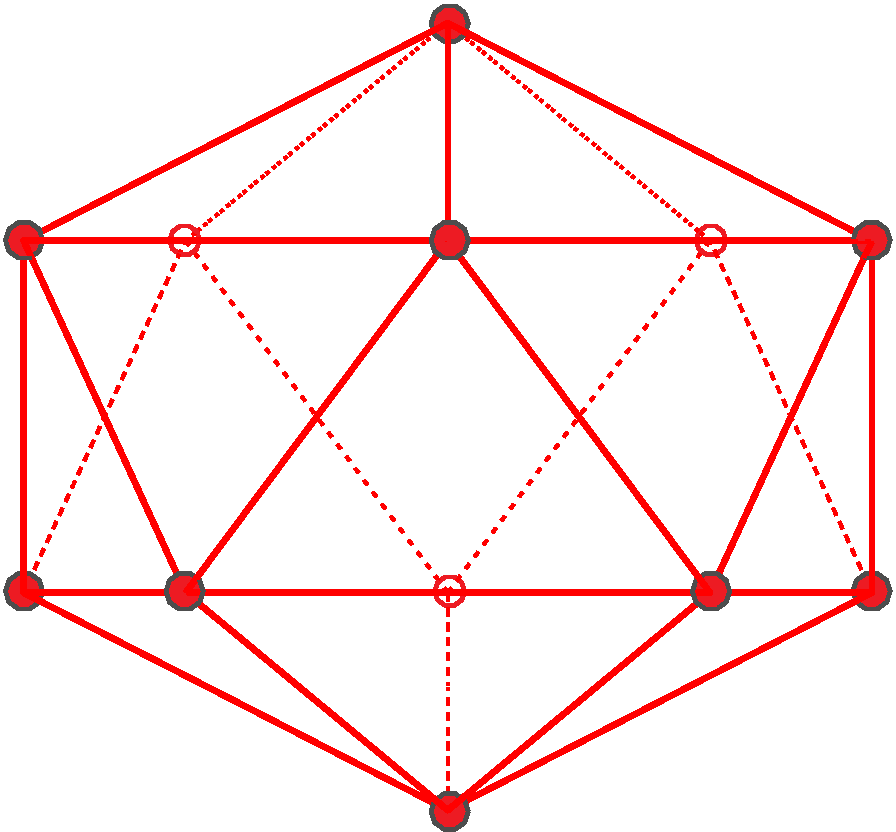
\includegraphics[width=\textwidth]{images/p_arr_construction_1.pdf}
		\caption{Start with icosahedron, created by applying icosahedral symmtry on one vector. Mathematically this is \(\mathcal{I}\vec{v}\).}
	\end{subfigure}
	\hfill
	\begin{subfigure}{0.3\textwidth}
		\centering
		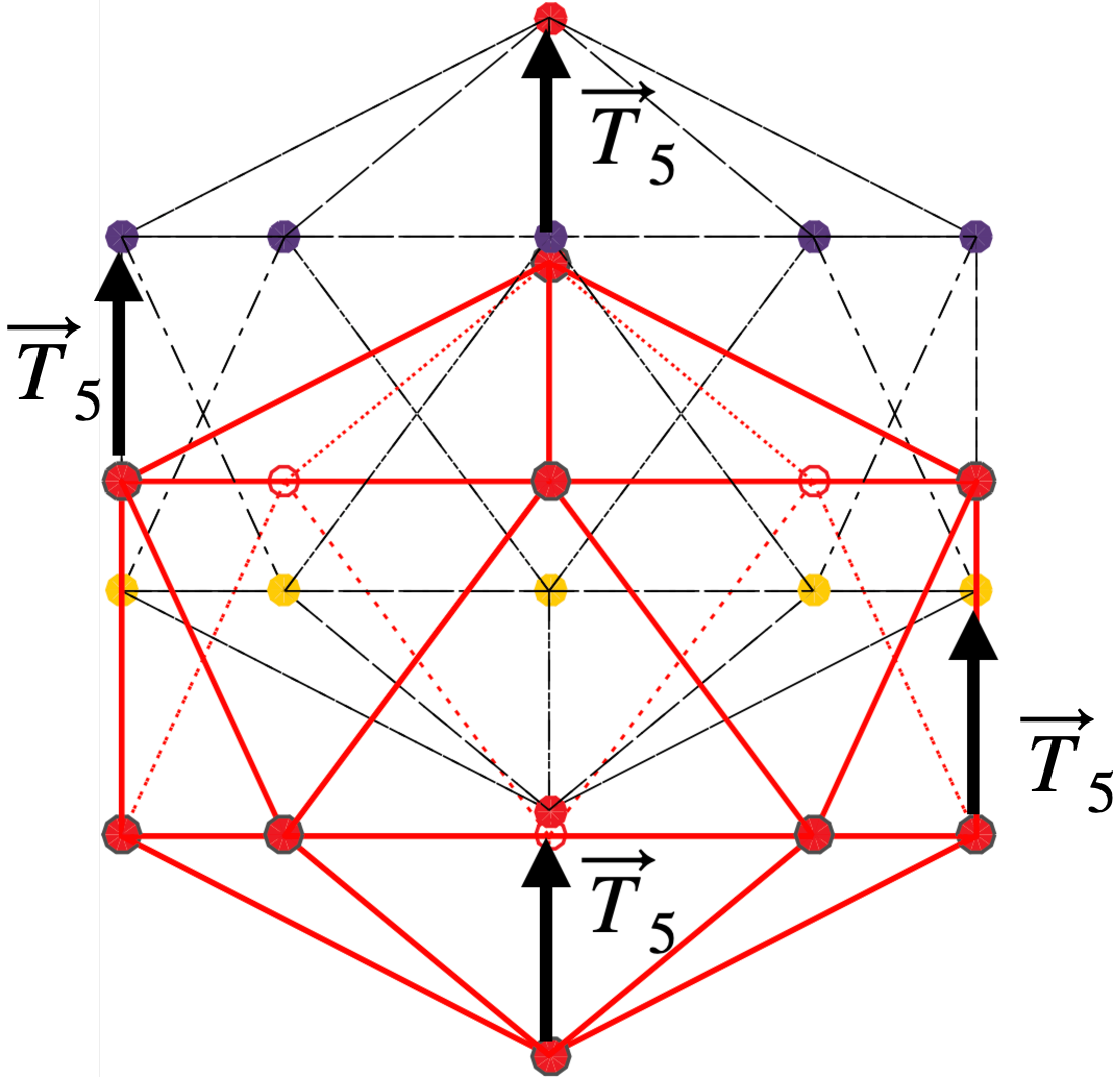
\includegraphics[width=\textwidth]{images/p_arr_construction_2.pdf}
		\caption{Shift icosahedron by a translation vector. In this example we are translating along the 5-fold axis of the icosahedron. Mathematically this is \mbox{\(\mathcal{I}\vec{v} \cup (\mathcal{I}\vec{v} + \vec{t})\)}.}
	\end{subfigure}
	\hfill
	\begin{subfigure}{0.35\textwidth}
		\centering
		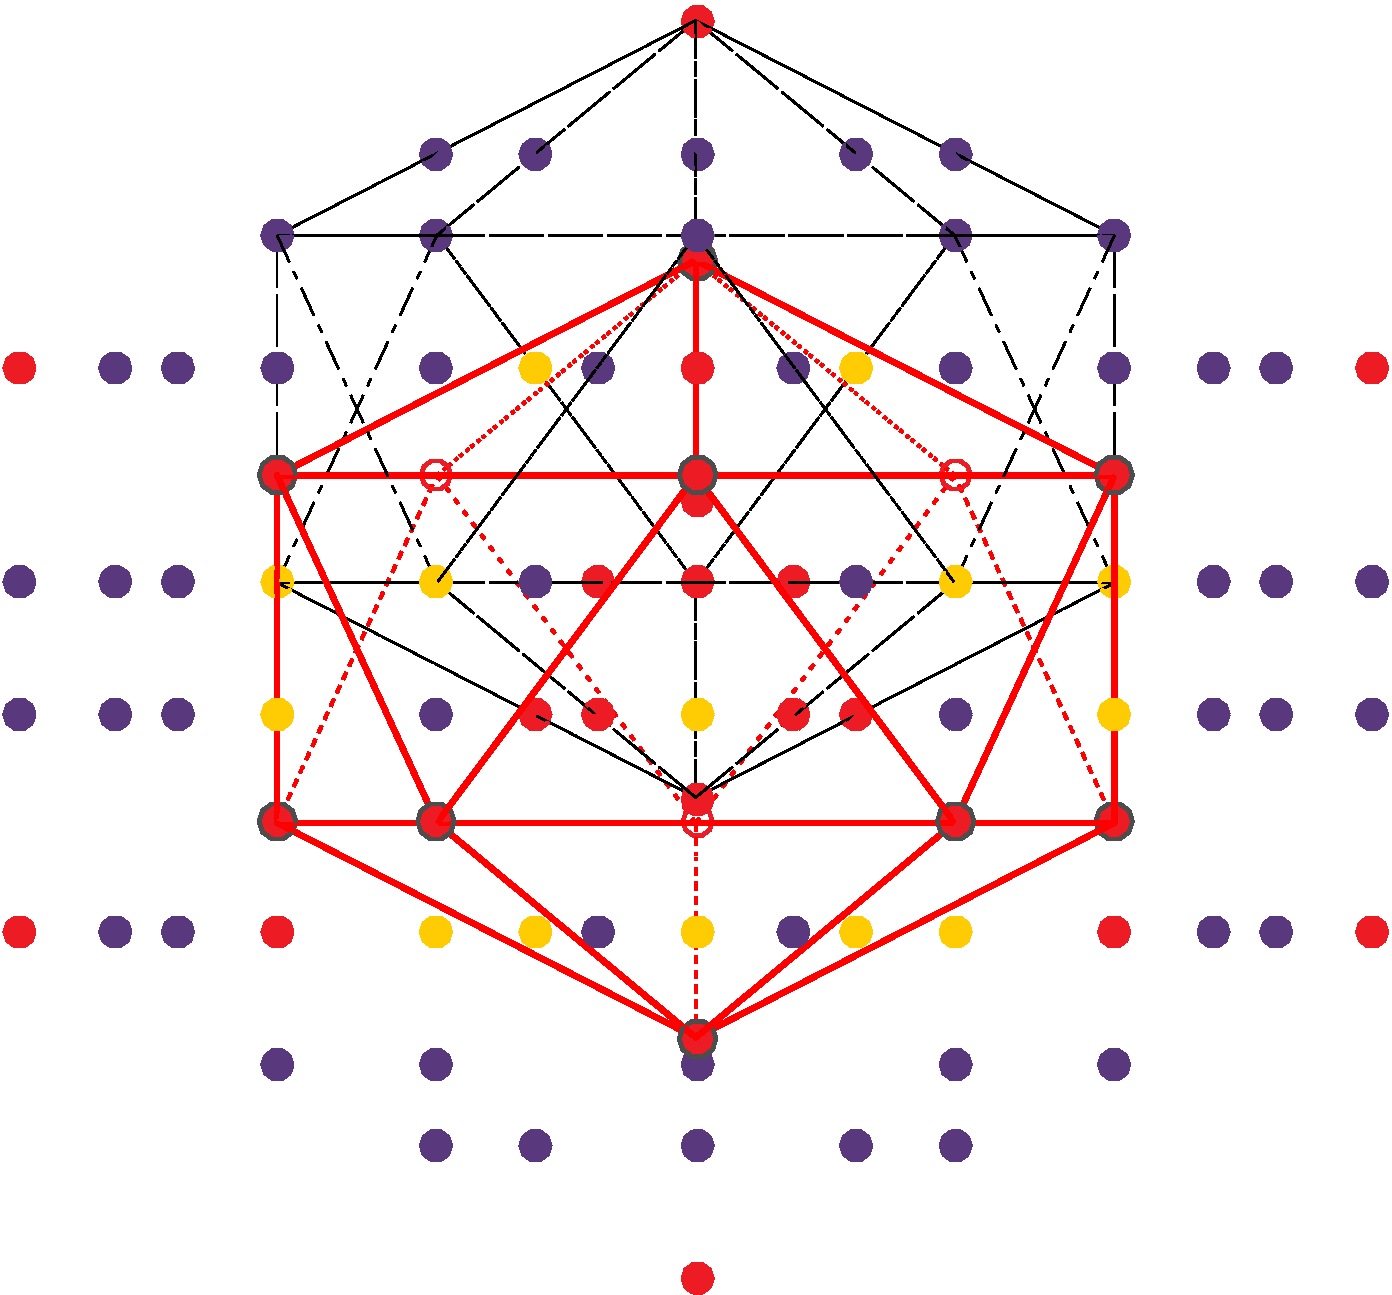
\includegraphics[width=\textwidth]{images/p_arr_construction_3.pdf}
		\caption{Reapply icosahedral symmetry, creating our one-base point array and getting the final expression \(\mathcal{I}\vec{v} \cup (\mathcal{I}\vec{v} + \mathcal{I}\vec{t})\).}
	\end{subfigure}
	\caption{The process of creating a one-base point array. Graphics from Dr. Dave Wilson.}
	\label{fig:point_array_construction}
\end{figure}

Here we define these one-base point arrays with two vectors, a translation and base vector.
However, we could define the same point array with more than two vectors, if we added on a vector from the base vector's icosahedral orbit.
Thus if \( \vec{u} \in \mathcal{I}\vec{v} \) we would have that 
\begin{equation}
	\mathcal{I}\vec{v} \cup (\mathcal{I}\vec{v} + \mathcal{I}\vec{t}) = \mathcal{I}\vec{v} \cup \mathcal{I}\vec{u} \cup (\mathcal{I}\vec{v} + \mathcal{I}\vec{t}) \cup (\mathcal{I}\vec{u} + \mathcal{I}\vec{t}).
	\label{eq:example-for-generating-lists}
\end{equation}
Therefore we have many ways of talking about the same point array.
\footnote{
	A quick proof for equation \ref{eq:example-for-generating-lists}:
	Let \( \text{LHS} = \mathcal{I}\vec{v} \cup (\mathcal{I}\vec{v} + \mathcal{I}\vec{t})\) and \( \text{RHS} = \mathcal{I}\vec{v} \cup \mathcal{I}\vec{u} \cup (\mathcal{I}\vec{v} + \mathcal{I}\vec{t}) \cup (\mathcal{I}\vec{u} + \mathcal{I}\vec{t})\)
	It is obvious that \( \text{LHS} \subseteq \text{RHS} \).
	Now take an element of the right hand side.
	Let \( x \in \text{RHS} \).
	If \( x \in \mathcal{I}\vec{v} \cup (\mathcal{I}\vec{v} + \mathcal{I}\vec{t}) \) we trivially have \( x \in \text{LHS} \).
	So first let \( x \in \mathcal{I}\vec{u} \).
	Then there exists \( G \in \mathcal{I} \) such that \( x = G\vec{u} \).
	Since \( \vec{u} \in \mathcal{I}\vec{v} \) then there exists \( H \in \mathcal{I} \) such that \( \vec{u} = H\vec{v} \).
	Thus \( x = GH\vec{v} \implies x \in \mathcal{I}\vec{v}\).
	Using the same idea, we get that \( x \in (\mathcal{I}\vec{u} + \mathcal{I}\vec{t}) \implies x \in (\mathcal{I}\vec{v} + \mathcal{I}\vec{t}) \).
	Therefore \( \text{LHS} \supseteq \text{RHS} \).
	We get equality by double inclusion.
}
\begin{Definition}[Minimal Generating List]
	A list of six dimensional vectors $ (\vec{t}, \vec{v}_1, \vec{v}_2, ... , \vec{v}_{n})$ is a \emph{minimal generating list}  and the union 
	\[
	\lpa{\vec{t}, \vec{v}_1, \vec{v}_2, ... , \vec{v}_{n}}: = \left(\bigcup_{i=1}^{n} \mathcal{I} \; \vec{v}_i \right) \cup \left( \bigcup_{i=1}^{n} \mathcal{I} \; \vec{v}_i + \mathcal{I} \; \vec{t} \right) 
	\]
	is called the \emph{($n$-base) lifted point array} generated by this list so long as 
	\begin{enumerate}
		\item Each of the vectors $\vec{t}$, $\vec{v}_i$ in the list points along a $2$-fold, $3$-fold or $5$-fold rotational axis of the action of $\mathcal{I}$.
		\item The orbits $\mathcal{I} \; \vec{v}_i$, $\; 1 \leq i \leq n$, are all distinct.
		\item We have the \emph{strict} inequality $\displaystyle 
		|\lpa{\vec{t}, \vec{v}_1, \vec{v}_2, ... , \vec{v}_{n}}| < \sum_{i=1}^{n} | \mathcal{I} \; \vec{v}_i| + | \mathcal{I} \; \vec{v}_i|| \mathcal{I} \; \vec{t}|. 
		$
	\end{enumerate}
	We say that a lifted point array is \emph{minimally generated} by \( (\vec{t}, \vec{v}_1, \vec{v}_2, ... , \vec{v}_{n}) \) if this list is a minimal generating list.
	\footnote{
		When looking at the 3rd condition for an $n$-base lifted point array, it may seem like we trivially have this condition.
		However, it is not trivial because we require a strict inequality.
		What this condition tells us is that the translated icosahedral orbits must intersect in some way.
		That is, there must exist \( G, H \in \mathcal{I} \) such that the sets \( \mathcal{I}\vec{v} + G\vec{t} \) and \( \mathcal{I}\vec{v} + H\vec{t} \) have a nonempty intersection.
	}
\end{Definition}
\begin{Definition}[Generating List]
	More generally, a list $ (\vec{t}, \vec{v}_1, \vec{v}_2, ... , \vec{v}_{n})$ is a \emph{generating list} if it has a sub-list $ (\vec{t}, \vec{v}_{i_1}, \vec{v}_{i_2}, ... , \vec{v}_{i_m})$, $1 \leq i_1 < i_2 < ... < i_m \leq n$, that is a minimal generating list and the unions
	\[
	\lpa{\vec{t}, \vec{v}_1, \vec{v}_2, ... , \vec{v}_{n}}: = \left(\bigcup_{i=1}^{n} \mathcal{I} \; \vec{v}_i \right) \cup \left( \bigcup_{i=1}^{n} \mathcal{I} \; \vec{v}_i + \mathcal{I} \; \vec{t} \right) 
	\]
	and $\lpa{\vec{t}, \vec{v}_{i_1}, \vec{v}_{i_2}, ... , \vec{v}_{i_m}}$ are equal.
\end{Definition}
% above two definitions are from Dr. Oloo
These definitions allow us to distinguish between the two cases given in equation \vref{eq:example-for-generating-lists}.
In that example the list \( (\vec{t}, \vec{v}) \) is the minimal generating list and the list \( (\vec{t}, \vec{v}, \vec{u}) \) is simply a generating list (assuming \( \vec{u} \in \mathcal{I}\vec{v} \)).

\subsection{Transitions Between Point Arrays}
Let us take an overall look at how we wish to use point arrays and their lifted counterparts.
Viruses are characterized by 3-dimensional point arrays.
We want our point arrays to represent the symmetry and structure of the virus.
We then lift the point arrays into 6 dimensions, because we want the point array to fit inside an icosahedral lattice.
Lattices on a general level encode symmetry (in particular they have both rotational and translational symmetry).
We will go more into depth about lattices in section \ref{section:lattices}.
By understanding the lattice structure, we can use the symmetries of a lattice in order to describe symmetry of the point array.
\todo{Add citation}
Point arrays let us look at the most important structural points of a virus and can determine what potential modifications could be done to a particular virus.

With point arrays, we can try to find linear transformations that map one point array onto another.
These transformations represent how a virus's structure changes over time.
In general, finding such a linear map is relatively easy.
A more difficult challenge is to find such a linear map that preserves symmetry.
Our point arrays have icosahedral symmetry.
Therefore our desire is to find a linear map from one point array to another where the intermediate point arrays also have icosahedral symmetry.
It may also be desirable to find a map that preserves the symmetries of one of the maximal subgroups of \( \mathcal{I} \) in cases where we cannot find a transition that preserves all of icosahedral symmetry.

Additionally, instead of mapping the point arrays directly onto each other, our linear transformations will transform one lattice into another.
The consequence of doing this is that when we restrict our map to the point array, it becomes a map from one point array to another.
The process of mathematically describing these symmetry preserving maps and how we find them will be the focus of the rest of this paper.
However, before we delve into the mathematics, we take a quick look at an example of virus that will be relevant to us.
\subsection{Viral Maturation}
Icosahedral viruses mature over time, and maturation is how they become infectous.
For this paper we will focus on the Cowpea Chlorotic Mottle Virus (CCMV).
This virus is characterized by one of the standard point arrays.
\footnote{
	The native state is characterized by the one-base point array $10$ and the mature state is characterized by the one-base point array $27$.
	See section \ref{section:all-one-base-point-arrays} for the definitions of these point arrays.
}
How CCMV matures is shown in figure \vref{fig:CCMV_maturation}.
Notice the points in orange, these points collectively are the point arrays that characterize the CCMV virus.
We wish to see if there exists a linear transformation that maps the native point array to the mature point array while preserving icosahedral symmetry (or one of its maximal subgroups).

\begin{figure}[!h]
	\centering
	\captionsetup{width=0.5\textwidth}
	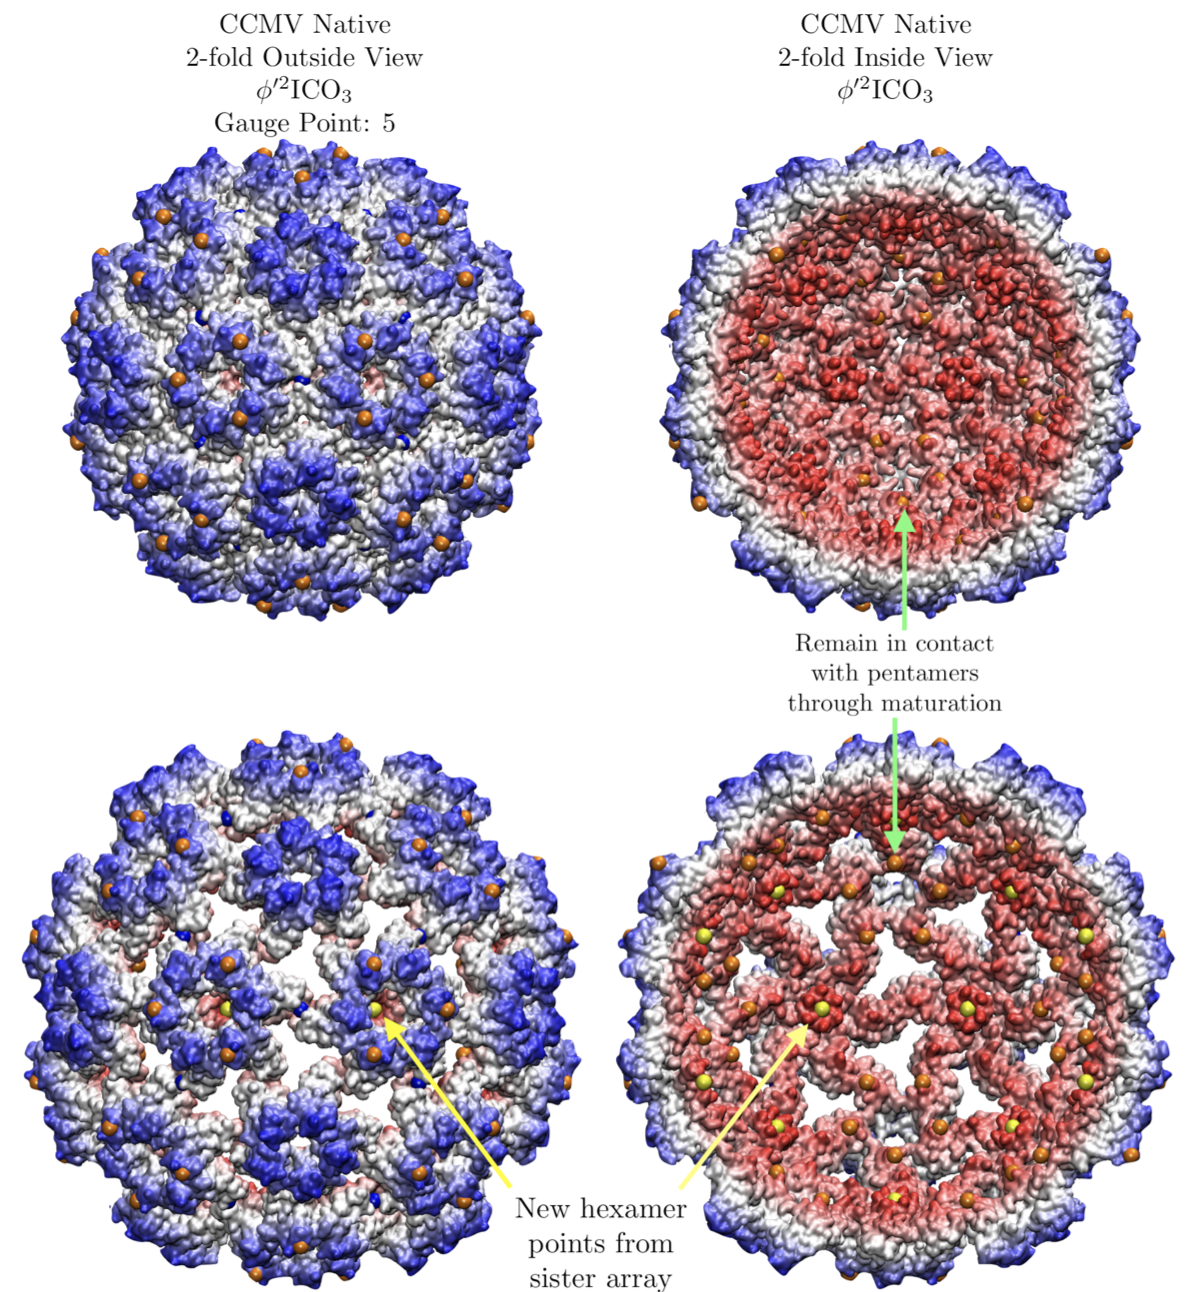
\includegraphics[width=0.5\textwidth]{images/CCMV_maturation.png}
	\caption{
		The above diagram shows CCMV in its native state (first row) and mature state (second row). 
		Notice the points in orange are the points that characterize CCMV.
		Graphics from Dr. Dave Wilson.
	}
	\label{fig:CCMV_maturation}
\end{figure}

\section{Mathematical View of the Problem}
Our desire is to find transitions between point arrays that preserves some form of icosahedral symmetry.
In order to find such transitions, we need to understand this problem mathematically.
On the highest level of abstraction, we are simply solving matrix equations of the form \[TB_0 = B_1.\]
In this equation, \(B_0\) and \(B_1\) represent the native and mature point arrays respectively, and \(T\) is our desired linear transformation that preserves icosahedral symmetry.
\footnote{Recall that we realize icosahedral symmetry as a matrix group and lifted point arrays are sets of vectors, so it makes sense that we are solving a matrix equation.}
Because we want to represent the point arrays, there is a specific structure to the \( B_0 \) and \( B_1 \) matrices.
Let us call us these matrices \emph{point array matrices}.
Before we define a point array matrix, we introduce a new notation called \emph{bar notation}.

\begin{Definition}[Icosahedral Bar Notation]
	Let \(\vec{v}\) be a 6-dimensional vector.
	Then we define that \(\overline{\vec{v}}\) is an element of the icosahedral orbit of \(\vec{v}\).
	That is, \(\overline{\vec{v}} \in \mathcal{I}\vec{v}\).
\end{Definition}
This definition allows us to easily denote when we wish to represent an element of the icosahedral orbit of a vector.
With this notation in hand, we can now define a point array matrix.
\begin{Definition}[Point Array Matrix]
	Let \(P\) be a given point array such that \( P \) is minimally generated by \( (\vec{t}, \vec{v}_1, \vec{v}_2, \dots, \vec{v}_n) \).
	A \emph{point array matrix} is a \( 6 \times (n+1) \) matrix of the form \[\begin{bmatrix}
		| & | & | & \cdots & | \\
		\overline{\vec{t}} & \overline{\vec{v}_1} & \overline{\vec{v}_2} & \cdots & \overline{\vec{v}_n} \\
		| & | & | & \cdots & | 
	\end{bmatrix}\]
	whose rank is either equal to the minimum of \( n+1 \) and 6.
	Notice that because we are using the icosahedral bar notation defined earlier, this definition is representing a class of matrices that all correspond to the same point array.
	That is, we are defining the form of any representative of the given point array \( P \).
	We denote the set of point array matrices for \( P \) as \( \pam(P) \).
\end{Definition}
The \( B_0 \) and \( B_1 \) matrices are both point array matrices and so both have this general form for their respective point arrays.

One fact that will be useful to know is how many point array matrices there are for a singular point array.
Let \( P \) be a point array.
If we let \( m \) be the number of point array matrices for \( P \) then
\[m \approx \abs{\mathcal{I}\vec{t}} \cdot \abs{\mathcal{I}\vec{v}_1} \cdot \abs{\mathcal{I}\vec{v}_2} \cdot \dots \cdot \abs{\mathcal{I}\vec{v}_n}.\]
We can only say for certain that \( m \) is less than or equal to this value because we require point array matrices to be linearly independent (or have rank 6).
\footnote{If we have that \( \vec{t} = \vec{v}_i \) for some \( i \), then there are matrices of the correct form that are not linearly independent.}
However, in general, we can assume that \( m \) is equal to this value since all the generating vectors are distinct.

\subsection{Lattices} \label{section:lattices}
In order to understand the nature of the transition matrix, we must understand lattices and how point arrays work with them.
For our point arrays, we use 6-dimensional icosahedral lattices.
First a definition:
\begin{Definition}[Bravais Lattice] \label{definition:bravais-lattice}
	A \emph{Bravais lattice} in $\mathbb{R}^n$ is the integer span of $n$ linearly independent vectors; the Bravais lattice generated by linearly independent vectors $\vec{a}_1, \vec{a}_2, ... , \vec{a}_n $ is
	 \[ \mathcal{L} := \{k_1\vec{a}_1 + k_2\vec{a}_2 + \dots + k_n\vec{a}_n \mid k_i \in \mathbb{Z}\} \]
\end{Definition}
Our point arrays fit inside this kind of lattice.
Lattices are interesting because of their discrete structure.
Let us consider three 2-dimensional examples, shown in figure \vref{fig:2d-lattice-examples}, that help explain two important invariants of lattices: the point group and the lattice group.
% 2D lattice examples
\begin{figure}[h]
	\centering
	\captionsetup{width=0.8\textwidth}
	% square lattice
	\begin{subfigure}{0.32\textwidth}
		\centering
		\begin{adjustbox}{width=0.9\textwidth}
		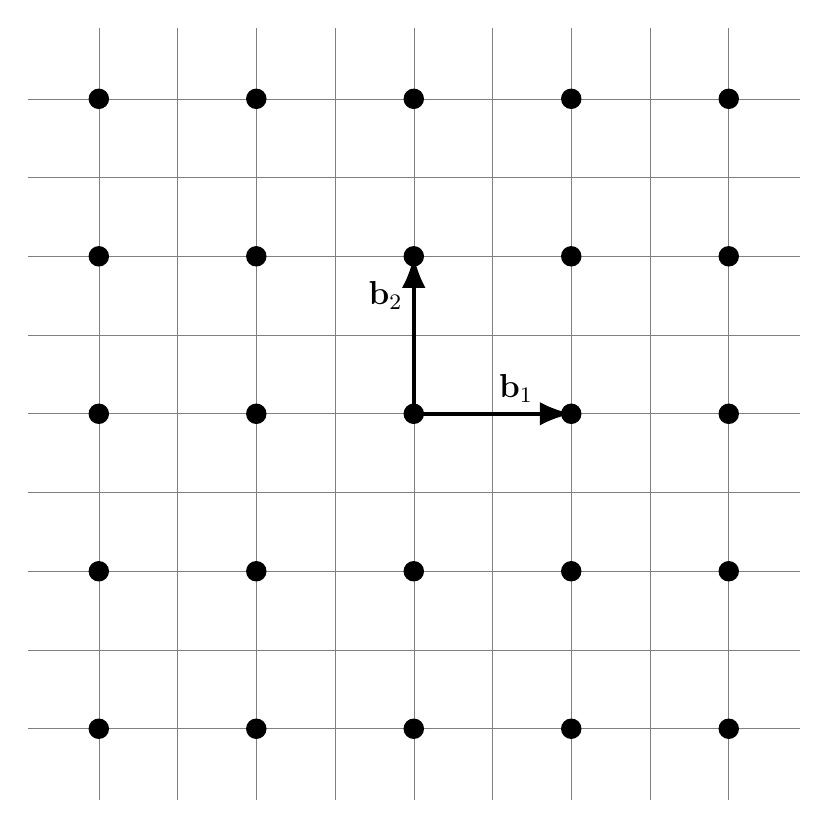
\begin{tikzpicture}
			\draw[step=1cm,gray,very thin] (-4.9,-4.9) grid (4.9,4.9);
			% square
			\foreach \x in {-4, -2, ..., 4}
				\foreach \y in {-4, -2, ..., 4}
					\fill (\x,\y) circle (0.13cm);
			
			% basis vectors
			\draw[-{Latex[length=4mm]}, line width=0.5mm] (0,0) -- (0,2) node[pos=0.75, left, font=\large]{\( \vec{b}_2 \)};
			\draw[-{Latex[length=4mm]}, line width=0.5mm] (0,0) -- (2,0) node[pos=0.65, above, font=\large]{\( \vec{b}_1 \)};
		\end{tikzpicture}
		\end{adjustbox}
		\caption{Square Lattice}
	\end{subfigure}
	% rectangular lattice
	\begin{subfigure}{0.32\textwidth}
		\centering
		\begin{adjustbox}{width=0.9\textwidth}
			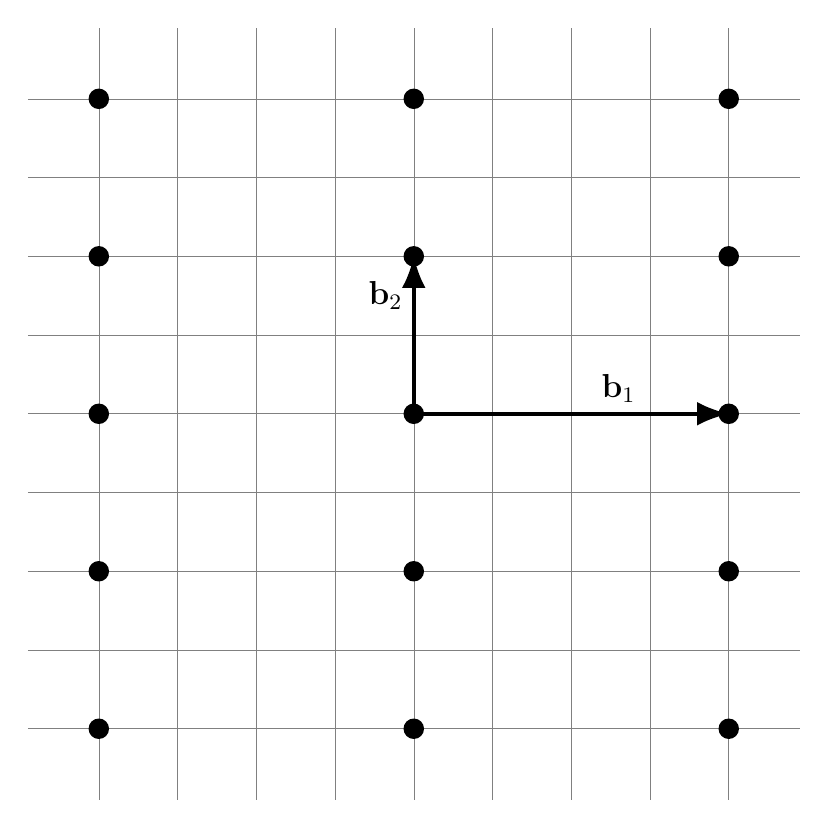
\begin{tikzpicture}
				\draw[step=1cm,gray,very thin] (-4.9,-4.9) grid (4.9,4.9);
				% rectangle
				\foreach \x in {-4, 0, 4}
					\foreach \y in {-4, -2, ..., 4}
						\fill (\x,\y) circle (0.13cm);
						
				% basis vectors
				\draw[-{Latex[length=4mm]}, line width=0.5mm] (0,0) -- (0,2) node[pos=0.75, left, font=\large]{\( \vec{b}_2 \)};
				\draw[-{Latex[length=4mm]}, line width=0.5mm] (0,0) -- (4,0) node[pos=0.65, above, font=\large]{\( \vec{b}_1 \)};
			\end{tikzpicture}
		\end{adjustbox}
		\caption{Rectangular Lattice}
	\end{subfigure}
	% centered rectangular lattice
	\begin{subfigure}{0.32\textwidth}
		\centering
		\begin{adjustbox}{width=0.9\textwidth}
			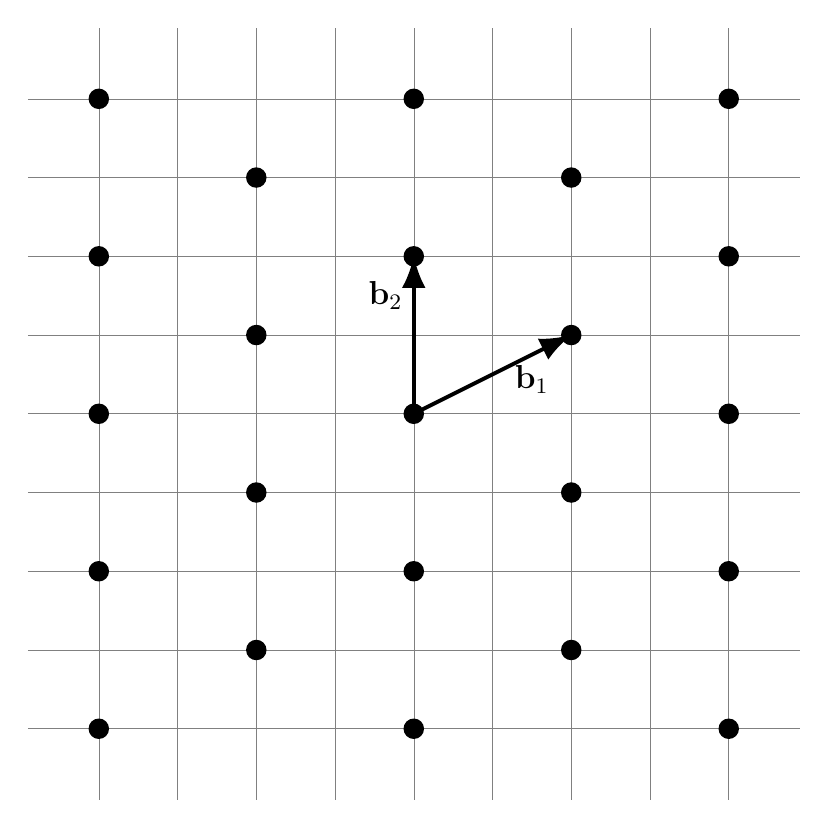
\begin{tikzpicture}
				\draw[step=1cm,gray,very thin] (-4.9,-4.9) grid (4.9,4.9);
				% rectangles
				\foreach \x in {-4, 0, 4}
					\foreach \y in {-4, -2, ..., 4}
						\fill (\x,\y) circle (0.13cm);
				% center dots
				\foreach \x in {-2, 2}
					\foreach \y in {-3, -1, 1, 3}
						\fill (\x,\y) circle (0.13cm);
						
				% basis vectors
				\draw[-{Latex[length=4mm]}, line width=0.5mm] (0,0) -- (0,2) node[pos=0.75, left, font=\large]{\( \vec{b}_2\)};
				\draw[-{Latex[length=4mm]}, line width=0.5mm] (0,0) -- (2,1) node[pos=0.75, below, font=\large]{\( \vec{b}_1 \)};
			\end{tikzpicture}
		\end{adjustbox}
		\caption{Centered Rectangular Lattice}
	\end{subfigure}
	\caption{Examples of 2-dimensional lattices. The grid represents standard integer coordinates for all three lattices. The basis vectors for each are labeled as \( \vec{b}_1 \) and \( \vec{b}_2 \).}
	\label{fig:2d-lattice-examples}
\end{figure}
\begin{Definition}[Point Group]
	The point group of a lattice \( \mathcal{L} \), denoted \( \mathcal{P}(\mathcal{L}) \), is the set of all orthogonal transformations that leave \( \mathcal{L} \) invariant.
	\footnote{Orthogonal transformations can be thought as distance preserving linear transformations that keeps the origin fixed.}
\end{Definition}
Let us determine the point group of our three example lattices.
For all three example lattices, we have two types of orthogonal transformations that leave the lattice invariant: rotations and reflections.
In the case of the square lattice, we have 4 reflections (reflections over the $x$-axis, $y$-axis, and the lines \( y = x \) and \( y = -x \)) and 4 rotations (rotate by either \( 0^\circ, 90^\circ, 180^\circ, \text{ or } 270^\circ \)).
These 8 transformations are the point group for the square lattice.
For both the rectangular and centered rectangular, we have 2 reflections (reflections over the $x$ and $y$ axes) and 2 rotations (rotate by either \( 0^\circ \text{ or } 180^\circ \)).
These four transformations are the point group for both the rectangular and centered rectangular lattices.
The point group gives us a coarse classification of lattices, in this case enabling us to distinguish the square lattice from the rectangular ones due to the non-isomorphic point groups.

Despite the rectangular and centered rectangular lattices having the same point group we notice that the fundamental structure of the two lattices are different.
Therefore there must be some way to distinguish them from each other by some other mathematical structure different from the point group. This finer classification is given by the lattice group, which combines the point group and basis vectors together.
\begin{Definition}[Lattice Group]
	Let \( B \) be a basis matrix
	\footnote{
		That is, \( B = \begin{bmatrix}
			| & | & \dots & | \\
			\vec{b}_1 & \vec{b}_2 & \dots & \vec{b}_n \\
			| & | & \dots & |
		\end{bmatrix} \)
		where \( \vec{b}_1, \vec{b}_2, \dots, \vec{b}_n \) are basis vectors.
	}
	for a lattice \( \mathcal{L} \).
	Then the lattice group, $\Lambda(B)$, consists of the representations of the elements of $\mathcal{P}(\mathcal{L})$ in this chosen basis. That is,
	\[\Lambda(B) := \{ N \in \Gl(n,\mathbb{Z}) \mid BN = MB \;\; \text{ for some } \; M \in \mathcal{P}(\mathcal{L})\}\]
	where $\Gl(n,\mathbb{Z})$ is the set of invertible $n \times n$ matrices with integer entries, and in fact
	\[\Lambda(B) = B^{-1} \; \mathcal{P}(\mathcal{L}) \; B.\]
\end{Definition}
In order to understand this definition, we will compute the lattice groups for the rectangular and centered rectangular lattices.
First, since transformations of 2-dimensional space can be thought of as \( 2 \times 2 \) matrices, we will express the point groups in this form.
Let \( R \) be the rectangular lattice and \( CR \) be the centered rectangular lattice.
Then
\begin{equation*}
	\mathcal{P}(R) = \mathcal{P}(CR) = \left\{
	\begin{bmatrix}
		1 & 0 \\
		0 & 1
	\end{bmatrix},
	\begin{bmatrix}
		-1 & 0 \\
		0 & -1
	\end{bmatrix},
	\begin{bmatrix}
		-1 & 0 \\
		0 & 1
	\end{bmatrix},
	\begin{bmatrix}
		1 & 0 \\
		0 & -1
	\end{bmatrix}
	\right\}
\end{equation*}
This set gives the matrix representations of rotation by $0^\circ$, rotation by $180^\circ$, reflection over the $y$-axis and reflection over the $x$-axis respectively.
In order to compute the lattice group, we first need the basis matrix for both lattices:
\begin{gather*}
	B_R = \begin{bmatrix}
		4 & 0 \\
		0 & 2
	\end{bmatrix} 
	\quad
	B_{CR} = \begin{bmatrix}
		2 & 0 \\
		1 & 2
	\end{bmatrix}
\end{gather*}
Now in order to compute the lattice groups \( \Lambda(R) \) and \( \Lambda(CR) \), we will solve the equations \( B_RN = MB_R \) and \mbox{\( B_{CR}N = MB_{CR} \)} for \( N \) for each \( M \) in the point group.
% showing computations in order to get lattice group
\begin{table*}[h]
	\centering
	\begin{adjustbox}{width=\textwidth}	
		\(\begin{array}{c|c}
			\Lambda(R) & \Lambda(CR)\\
			\hline
			\\
			% row 1
			\begin{bmatrix}
				4 & 0 \\
				0 & 2
			\end{bmatrix}
			\cdot N
			=
			\begin{bmatrix}
				1 & 0 \\
				0 & 1
			\end{bmatrix}
			\begin{bmatrix}
				4 & 0 \\
				0 & 2
			\end{bmatrix}
			\implies N = 
			\begin{bmatrix}
				1 & 0 \\
				0 & 1
			\end{bmatrix}
			&
			\begin{bmatrix}
				2 & 0 \\
				1 & 2
			\end{bmatrix}
			\cdot N
			=
			\begin{bmatrix}
				1 & 0 \\
				0 & 1
			\end{bmatrix}
			\begin{bmatrix}
				2 & 0 \\
				1 & 2
			\end{bmatrix}
			\implies N = 
			\begin{bmatrix}
				1 & 0 \\
				0 & 1
			\end{bmatrix}
			\\\\
			% row 2
			\begin{bmatrix}
				4 & 0 \\
				0 & 2
			\end{bmatrix}
			\cdot N
			=
			\begin{bmatrix}
				-1 & 0 \\
				0 & -1
			\end{bmatrix}
			\begin{bmatrix}
				4 & 0 \\
				0 & 2
			\end{bmatrix}
			\implies N = 
			\begin{bmatrix}
				-1 & 0 \\
				0 & -1
			\end{bmatrix}
			&
			\begin{bmatrix}
				2 & 0 \\
				1 & 2
			\end{bmatrix}
			\cdot N
			=
			\begin{bmatrix}
				-1 & 0 \\
				0 & -1
			\end{bmatrix}
			\begin{bmatrix}
				2 & 0 \\
				1 & 2
			\end{bmatrix}
			\implies N = 
			\begin{bmatrix}
				-1 & 0 \\
				0 & -1
			\end{bmatrix}
			\\\\
			% row 3
			\begin{bmatrix}
				4 & 0 \\
				0 & 2
			\end{bmatrix}
			\cdot N
			=
			\begin{bmatrix}
				-1 & 0 \\
				0 & 1
			\end{bmatrix}
			\begin{bmatrix}
				4 & 0 \\
				0 & 2
			\end{bmatrix}
			\implies N = 
			\begin{bmatrix}
				-1 & 0 \\
				0 & 1
			\end{bmatrix}
			&
			\begin{bmatrix}
				2 & 0 \\
				1 & 2
			\end{bmatrix}
			\cdot N
			=
			\begin{bmatrix}
				-1 & 0 \\
				0 & 1
			\end{bmatrix}
			\begin{bmatrix}
				2 & 0 \\
				1 & 2
			\end{bmatrix}
			\implies N = 
			\begin{bmatrix}
				-1 & 0 \\
				1 & 1 
			\end{bmatrix}
			\\\\
			% row 4
			\begin{bmatrix}
				4 & 0 \\
				0 & 2
			\end{bmatrix}
			\cdot N
			=
			\begin{bmatrix}
				1 & 0 \\
				0 & -1
			\end{bmatrix}
			\begin{bmatrix}
				4 & 0 \\
				0 & 2
			\end{bmatrix}
			\implies N = 
			\begin{bmatrix}
				1 & 0 \\
				0 & -1
			\end{bmatrix}
			&
			\begin{bmatrix}
				2 & 0 \\
				1 & 2
			\end{bmatrix}
			\cdot N
			=
			\begin{bmatrix}
				1 & 0 \\
				0 & -1
			\end{bmatrix}
			\begin{bmatrix}
				2 & 0 \\
				1 & 2
			\end{bmatrix}
			\implies N = 
			\begin{bmatrix}
				1 & 0 \\
				-1 & -1 
			\end{bmatrix}
			\\
		\end{array}\)
	\end{adjustbox}
\end{table*}

\noindent These series of computations tell us what the lattice groups are:
% listing the lattice groups for R and CR
\begin{gather*}
	\Lambda(R) = \left\{
	\begin{bmatrix}
		1 & 0 \\
		0 & 1
	\end{bmatrix},
	\begin{bmatrix}
		-1 & 0 \\
		0 & -1
	\end{bmatrix},
	\begin{bmatrix}
		-1 & 0 \\
		0 & 1
	\end{bmatrix},
	\begin{bmatrix}
		1 & 0 \\
		0 & -1
	\end{bmatrix}
	\right\} \\
	\Lambda(CR) = \left\{
	\begin{bmatrix}
		1 & 0 \\
		0 & 1
	\end{bmatrix},
	\begin{bmatrix}
		-1 & 0 \\
		0 & -1
	\end{bmatrix},
	\begin{bmatrix}
		-1 & 0 \\
		1 & 1
	\end{bmatrix},
	\begin{bmatrix}
		1 & 0 \\
		-1 & -1
	\end{bmatrix}
	\right\}
\end{gather*}
%\todo{convince self that these lattice groups aren't \( \Gl(2, \Z) \) conjugate.}
Notice that the lattice groups for the rectangular and centered rectangular lattices are not \( \Gl(2, \Z) \) conjugate.
Because these lattice groups are not \( \Gl(2, \Z) \) conjugate, the structure of their corresponding lattices is fundamentally different.
So by using lattice groups, we can clearly distinguish between different lattices.

\begin{Remark*}
	%\todo[color=yellow]{This is straight ripped from the paper paper.}
	The lattice groups associated to bases of the same lattice may be different but they are always $\Gl(n,\mathbb{Z})$ conjugate. This is because if $B$, $B'$ are basis matrices of the same lattice then there is an invertible integer matrix $N$ such that 
	\[BN = B'.\]
\end{Remark*}
Now that we have explained the importance of the point and lattice groups using these 2D examples, we can define the 6-dimensional icosahedral lattices relevant to our point arrays.
We want the lattices in which our point arrays sit \sout{in} to be invariant under the icosahedral group \( \mathcal{I} \).
There are three 6-dimensional icosahedral lattices that are relevant to us:
\begin{align*}
	\mathcal{L}_{SC} &:= \{ (x_1,x_2, ...,x_n) \mid x_i \in \mathbb{Z} \} \\
	\mathcal{L}_{BCC} &:= \{ \textstyle \frac{1}{2}(x_1,x_2, ...,x_n) \mid x_i \in \mathbb{Z}, \; x_i \equiv x_j \; \text{mod } 2  \;\;\forall i,j \} \\
	\mathcal{L}_{FCC} &:= \{ \textstyle \frac{1}{2}(x_1,x_2, ...,x_n) \mid x_i \in \mathbb{Z}, \; x_1+x_2+...+x_6 \equiv 0 \; \text{mod } 2 \;\; \forall i,j \},
\end{align*}
which are referred to the standard simple cubic, body centered cubic, and face centered cubic lattices respectively.
Notice that \( \mathcal{L}_{SC} \subset \mathcal{L}_{BCC} \subset \mathcal{L}_{FCC} \).
All icosahedral lattices are equivalent to one of these three \cite{levitovrhyner1988crystallography}.
\footnote{Roughly speaking, two lattices are equivalent if their lattice groups are conjugate in \( \Gl(n, \Z) \).}
When considering our point arrays, we want to know which of these lattices they fit into best.
\begin{Definition}[Minimal Lattice]
	Let \( P \) be a lifted point array.
	A \emph{minimal lattice}, denoted \( \mathcal{L}_\mathcal{I}(P) \) is an icosahedral lattice containing \( P \) that is contained in every other icosahedral lattice containing \( P \).
\end{Definition}
A minimal lattice can also be thought of the smallest lattice that contains \( P \).
The following propositions (which we will state without proof) tells what the minimal lattice is for a set of points in 6-dimensions.
\begin{Proposition}[{\cite[Proposition 1]{indelicatoetal2012}}]
	Given vectors \( \vec{v}_1, \vec{v}_2, \dots, \vec{v}_n \in \R^6 \) all contained in some 6-dimensional icosahedral lattice \( \mathcal{L} \), the \( \Z \)-span of the union \( \mathcal{O} := \mathcal{I}\vec{v}_1 \cup \mathcal{I}\vec{v}_2 \cup \dots \cup \mathcal{I}\vec{v}_n \), which is defined as
	\[\mathcal{L}_\mathcal{I}(\vec{v}_1, \vec{v}_2, \dots, \vec{v}_n) := \left\{\sum_{\vec{w} \in \mathcal{O}} c_\vec{w}\vec{w} \;\bigg|\; c_\vec{w} \in \Z \right\},\]
	is the minimal icosahedral lattice containing the vectors \( \vec{v}_1, \vec{v}_2, \dots, \vec{v}_n \).
\end{Proposition}
\begin{Proposition}[{\cite[Proposition 1]{indelicatoetal2012}}]
	If a lifted point array is generated by the vectors \( \vec{t}, \vec{v}_1, \vec{v}_2, \dots, \vec{v}_n \), then the minimal lattice containing that point array is \( \mathcal{L}_\mathcal{I}(\vec{t}, \vec{v}_1, \vec{v}_2, \dots, \vec{v}_n) \).
\end{Proposition}

\subsection{Transitions Between Lifted Point Arrays}
Now that we have an understanding of lattices, we have the tools necessary to mathematically describe our symmetry preserving transformations between point arrays.
The symmetries of our point arrays are encoded within its minimal lattice and its corresponding lattice group.
Thus we want our linear transformations to not only be a map from one point array to another, but also a map of their minimal lattices that will preserve some form of symmetry (in our case it will be a subgroup of \( \mathcal{I} \)).
The following definition gives us a description of a transformation that does this.
\begin{Definition}[Definitions 4 and 5 from \cite{indelicatoetal2012}]
	\label{def:transitions-indelicato}
	Let \( \mathcal{L}_0 \) and \( \mathcal{L}_1 \) be icosahedral lattices and \( \mathcal{G}_0 \) be a subgroup of \( \mathcal{I} \).
	\begin{enumerate}
		\item A \emph{transition} from \( \mathcal{L}_0 \) and \( \mathcal{L}_1 \) with intermediate symmetry \( \mathcal{G}_0 \) is a continuous function \begin{gather*}
			\mathcal{B}\colon [0, 1] \to \Gl(n, \R) \\
			\sigma \mapsto \mathcal{B}_\sigma
		\end{gather*}
		such that \( \mathcal{B}_0 \) is a basis matrix of \( \mathcal{L}_0 \), \( \mathcal{B}_1 \) is a basis matrix of \( \mathcal{L}_1 \), and letting
		\[\mathcal{G} := B_0^{-1}\mathcal{G}_0\mathcal{B}_0 \subset \Lambda(\mathcal{B}_0)\]
		we have
		\[\mathcal{G} \subset \Lambda(\mathcal{B}_\sigma) \text{ for all } \sigma \in [0, 1].\]
		
		\item Additionally a transition \( \mathcal{B} \) from \( \mathcal{L}_0 \) to \( \mathcal{L}_1 \) with intermediate symmetry \( \mathcal{G}_0 \) is compatible with projection if 
		\[\mathcal{B}_\sigma\mathcal{G}B_\sigma^{-1} \subset \mathcal{P}(\mathcal{L}(\mathcal{B}_\sigma)) \text{ for all } \sigma \in [0, 1].\]
	\end{enumerate}
	We refer to \[T(\sigma) := \mathcal{B}_\sigma \mathcal{B}_0^{-1} \quad\text{ and }\quad T := T(1) = \mathcal{B}_1\mathcal{B}_0^{-1}\] as the \emph{transition path} and the \emph{transition} respectively.
\end{Definition}
\noindent This definition tells us that our transitions from one lattice to another will have the following properties:
\begin{enumerate}
	\item All intermediate lattices have at least \( \mathcal{G}_0 \) symmetry;
	\item The intermediate lattices are actually \( \mathcal{G}_0 \) invariant.
\end{enumerate}
Additionally, because we want our transitions to both describe a continuous path and preserve \( \mathcal{G}_0 \) symmetry, it turns out that our transition must be in the centralizer of \( \mathcal{G}_0 \) \cite{indelicatoetal2012}.
\begin{Definition}[Centralizer]
	The centralizer of a group \(G\), denoted by \(Z(G)\) is the set of elements that commute with all elements of \(G\).
	That is, \[Z(G) = \{z\ |\ gz = zg\ \forall g \in G\}.\]
\end{Definition}
Since these transitions belong to the centralizer of our symmetry groups, the matrices that describe our transitions will also commute with the lattice's point group and lattice group.

\subsection{The Form of Transitions}
In the previous section, we built up the necessary background in order to arrive at the conclusion that our transitions must be in the centralizer of \( \mathcal{I} \) or in the centralizer of one its maximal subgroups.
Luckily for us, Indelicato et al. have explicitly calculated what the centralizers are for our symmetry groups \cite{indelicatoetal2012}.
Let's first start with the icosahedral group.
A transition \(T\) that preserves all of icosahedral symmetry must have the form: \begin{equation*}
	T = \begin{bmatrix}
		z  & x  & -x & -x & x  & x \\
		x  & z  & x  & -x & -x & x \\
		-x & x  & z  & x  & -x & x \\
		-x & -x & x  & z  & x  & x \\
		x  & -x & -x & x  & z  & x \\
		x  & x  & x  & x  & x  & z
	\end{bmatrix}
\end{equation*}
where \( x, z \in \R \).
Any matrix of the form given in the above equation is in \(Z(\mathcal{I})\), the centralizer of \(\mathcal{I}\), and thus mathematically describes a transition that preserves icosahedral symmetry.
Now we can look at the maximal subgroups of \( \mathcal{I} \).
Below are the general matrix forms for \(Z(A_4)\), \(Z(D_{10})\), and \(Z(D_6)\). \cite{indelicatoetal2012}
\begin{gather*}
	\begin{bmatrix}
		z  & -x & -y & -t & t  & -x \\
		t  & z  & t  & x  & x  & y  \\
		-y & -x & z  & t  & -t & -x \\
		x  & -t & -x & z  & y  & t  \\
		-x & -t & x  & y  & z  & t  \\
		t  & y  & t  & -x & -x & z
	\end{bmatrix} \in Z(A_4)
	\quad \quad
	\begin{bmatrix}
		z & x & y & y & x & t \\
		x & z & x & y & y & t \\
		y & x & z & x & y & t \\
		y & y & x & z & x & t \\
		x & y & y & x & z & t \\
		u & u & u & u & u & w
	\end{bmatrix} \in Z(D_{10}) \\
	\begin{bmatrix}
		u  & w  & -w & x  & s  & s  \\
		-t & y  & v  & -v & z  & -t \\
		t  & v  & y  & v  & t  & -z \\
		z  & -v & v  & y  & -t & -t \\
		s  & x  & -w & w  & u  & s  \\
		s  & w  & -x & w  & s  & u
	\end{bmatrix} \in Z(D_{6})
\end{gather*}
Similarly to \( Z(\mathcal{I}) \), we have that all of these variables represent real numbers.
These general matrix forms give us linear transformations that preserve the symmetry of one of the maximal subgroups.
Notice that with particular choices of variables, all three of these general forms can be equal to general form for icosahedral symmetry.
\footnote{
	For \( Z(A_4) \), choosing \( t = y = -x \) gives us the general form for \( Z(\mathcal{I}) \).
	For \( Z(D_{10}) \), choosing \( y = u = t = x \) and \( w = z \) gives us the general form for \( Z(\mathcal{I}) \).
	And for \( Z(D_6) \), choosing \( u = y \), \( x = t = z = -w \), and \( s = v = w \) gives us the general form for \( Z(\mathcal{I}) \).
}
This tells us that \( Z(\mathcal{I}) \) is a subset of the sets \( Z(A_4), Z(D_{10}), Z(D_6) \).

Definition \ref{def:transitions-indelicato} gives us a rigorous definition of a transition between point arrays. 
However, for the purposes of computing transitions between point arrays, we can vastly simplify our definitions.
For transition matrices, we will only need to work with the following definition, which we will be using for the rest of this paper.
\begin{Definition}[Transition Matrix]
	Let \(\mathcal{G} = \mathcal{I}, A_4, D_{10}, \text{or } D_6\).
	A \emph{transition matrix} that preserves intermediate symmetry \( \mathcal{G} \) is an invertible matrix 
	\footnote{
		Note that we require our transitions to be invertible matrices because if we find a transition matrix \( T \) for \( P \to Q \), we want to be guarenteed that \( T^{-1} \) is a transition for \( Q \to P \).
	}
	that is also an element of \( Z(\mathcal{G}) \).
\end{Definition}
\noindent Additionally while definition \ref{def:transitions-indelicato} requires us to find a continuous map from 0 to 1, we actually only need to find the final transition \( T \) in the transition path.
\footnote{
	The transition path describes a straight line, so if we have the final transition matrix we can simply create a continuous linear map from the identity matrix to \( T \).
}
By simplifying our definitions, it will give us a strong start in finding and computing transitions between point arrays.

\subsection{How To Find Transitions}
We now understand the mathematical structures of the problem.
The question now is what procedure should we use in order to find transitions that preserve symmetry.

Suppose we want to a symmetry preserving transition from point array \( P \) to point array \( Q \).
Then to find this transition, we need to find a point array matrix \( B_0 \in \pam(P) \) and a point array matrix \( B_1 \in \pam(Q) \) such that the equation \( TB_0 = B_1 \) can be solved for \( T \).
Thus we if wish to find a transition preserving icosahedral symmetry, then our equation looks like
\begin{equation}
	\begin{bmatrix}
		z  & x  & -x & -x & x  & x \\
		x  & z  & x  & -x & -x & x \\
		-x & x  & z  & x  & -x & x \\
		-x & -x & x  & z  & x  & x \\
		x  & -x & -x & x  & z  & x \\
		x  & x  & x  & x  & x  & z
	\end{bmatrix}
	\cdot
	\begin{bmatrix}
		| & | & | & \cdots & | \\
		\overline{\vec{t}} & \overline{\vec{v}_1} & \overline{\vec{v}_2} & \cdots & \overline{\vec{v}_n} \\
		| & | & | & \cdots & |
	\end{bmatrix}
	=
	\begin{bmatrix}
		| & | & | & \cdots & | \\
		\overline{\vec{t}'} & \overline{\vec{u}_1} & \overline{\vec{u}_2} & \cdots & \overline{\vec{u}_n} \\
		| & | & | & \cdots & |
	\end{bmatrix}
	\label{eq:general-ico-equation}
\end{equation}
where \( P \) is minimally generated by \((\vec{t}, \vec{v}_1, \vec{v}_2, \dots, \vec{v}_n)\) and \( Q \) is minimally generated by vectors \((\vec{t'}, \vec{u}_1, \vec{u}_2, \dots, \vec{u}_n)\).
\footnote{
	It is possible that \( P \) and \( Q \) are minimally generated by an unequal number vectors, which would cause this equation to be invalid. 
	There is a way to make the equation work when this is case and is described in section \ref{section:appendix-point-arrays}.
	\label{footnote:unequal-sized-point-arrays}
}
Because \( \pam(P) \) and \( \pam(Q) \) are sets of matrices, equation \vref{eq:general-ico-equation} describes a set of equations, whose cardinality is equal to \( \abs{\pam(P)}\cdot\abs{\pam(Q)}\).
Therefore, to find an icosahedral symmetry preserving transition, we must find an equation within this set that is solvable.
\footnote{
	One may notice that by how this equation is setup, the order of the generators matters.
	This is in constrast to the definition of an lifted point array, where the order doesn't matter.
	In truth, any permutation of the columns of both \( B_0 \) and \( B_1 \) is allowed (except for the first columns, which must remain first) and so the true number of equations is multiplied by \( n!^2 \).
	The true number of equations that must be checked for the transition \( P \to Q \) is \( n!^2\cdot\abs{\pam(P)}\cdot\abs{\pam(Q)} \).
	However, when we actually compute these transitions, we consider the various permutations of the generators as separate cases entirely and thus can forgo talking about permutations when finding transitions.
}

\subsection{CCMV \( D_6 \) Transition Example}
The following is an example of an equation for the CCMV virus the preserves \(D_6\) symmetry:
\begin{equation*}
	\renewcommand*{\arraystretch}{1.5}
	\begin{bmatrix}
		u  & w  & -w & x  & s  & s  \\
		-t & y  & v  & -v & z  & -t \\
		t  & v  & y  & v  & t  & -z \\
		z  & -v & v  & y  & -t & -t \\
		s  & x  & -w & w  & u  & s  \\
		s  & w  & -x & w  & s  & u
	\end{bmatrix}
	\cdot
	\begin{bmatrix}
		-\frac{1}{2} & -\frac{3}{2} \\
		-\frac{1}{2} & \frac{1}{2} \\
		\frac{1}{2} & -\frac{1}{2} \\
		-\frac{1}{2} & -\frac{1}{2} \\
		-\frac{1}{2} & \frac{1}{2} \\
		\frac{1}{2} & \frac{1}{2}
	\end{bmatrix}
	=
	\begin{bmatrix}
		0 & 0 \\
		0 & 0 \\
		-1 & 0 \\
		0 & -1 \\
		0 & -1 \\
		0 & -1 \\
	\end{bmatrix}
	\label{eq:ccmv_d6_example}
\end{equation*}
and simplifies to:
\begin{equation*}
	\renewcommand*{\arraystretch}{1.5}
	\begin{bmatrix}- \frac{u}{2} - w - \frac{x}{2} & s - \frac{3 u}{2} + w - \frac{x}{2}\\v - \frac{y}{2} - \frac{z}{2} & t + \frac{y}{2} + \frac{z}{2}\\- t - v + \frac{y}{2} - \frac{z}{2} & - t - \frac{y}{2} - \frac{z}{2}\\v - \frac{y}{2} - \frac{z}{2} & - t - v - \frac{y}{2} - \frac{3 z}{2}\\- \frac{u}{2} - w - \frac{x}{2} & - s + \frac{u}{2} + \frac{x}{2}\\- s + \frac{u}{2} - w - \frac{x}{2} & - s + \frac{u}{2} + \frac{x}{2}\end{bmatrix}
	=
	\begin{bmatrix}
		0 & 0 \\
		0 & 0 \\
		-1 & 0 \\
		0 & -1 \\
		0 & -1 \\
		0 & -1 \\
	\end{bmatrix}
	\label{eq:ccmv_d6_example_simplified}
	% solution to this equation is {s: 1, t: 0, u: 1, v: 0, w: 0, x: -1, y: -1, z: 1}
\end{equation*}
This equation can be solved and gives us the transition matrix:
\begin{equation*}
	T =
	\begin{bmatrix}
		1  & 0  & 0 & -1  & 1  & 1  \\
		0 & -1  & 0  & 0 & 1  & 0 \\
		0  & 0  & -1  & 0  & 0  & -1 \\
		1  & 0 & 0  & -1  & 0 & 0 \\
		1  & -1  & 0 & 0  & 1  & 1  \\
		1  & 0  & 1 & 0  & 1  & 1
	\end{bmatrix}
\end{equation*}
In this case, these particular \( B_0 \) and \( B_1 \) matrices make the equation such that it can be solved for \( T \).
However, there are many other choices for \( B_0 \) and \( B_1 \) for which the equation cannot be solved for \( T \).

\section{Computational Techniques} \label{section:computational-techniques}
In order to compute transition matrices, we need to generate all of the equations that could describe a transition from point array \( P \) to point array \( Q \), and then check if any of them can be solved.
Generating all of the possible equations is simple enough, as we can take the cartesian product of the icosahedral orbits of the generators.
That is, if \( P \) is minimally generated by \((\vec{t}, \vec{v}_1, \vec{v}_2, \dots, \vec{v}_n)\) and \( Q \) is minimally generated by vectors \((\vec{t'}, \vec{u}_1, \vec{u}_2, \dots, \vec{u}_n)\), then the each equation we need to solve corresponds to an element of the product
\[\mathcal{I}\vec{t} \times \mathcal{I}\vec{v}_1 \times \mathcal{I}\vec{v}_2 \times \dots \times \mathcal{I}\vec{v}_n \times \mathcal{I}\vec{t'} \times \mathcal{I}\vec{u}_1 \times \mathcal{I}\vec{u}_2 \times \dots \times \mathcal{I}\vec{u}_n.\]
So we just need to generate and loop over all elements of this cartesian product and check if the equation is solvable.
This description of how to solve the problem is the brute force approach.
While the approach will give us the answer we desire, it may be very slow in finding transitions, especially if \( n \geq 3 \) since the size of the cartesian product grows exponentially with \( n \).
\footnote{
	The size of the icosahedral orbit of a 6-dimensional vector could in theory be any factor of 60, however in application they have sizes 12, 20, and 30.
	If we assume they have all of size 20, then when \( n = 3 \), the size of the cartesian product is \( 20^{2(n+1)} = 25,600,000,000 \).
	This is infeasible for any computer to fully check in a reasonable amount of time.
}

Despite this, we can speed up this computation even with this brute force approach through parallelization.
We can parallelize this problem because each matrix equation is independent of every other equation.
Thus each element of our cartesian product is an independent task that needs to be completed.
Because this problem is easily parallelizable, it known as \emph{embarassingly parallel}.
\begin{Definition}[Embarassingly Parallel \cite{Pacheco_2011}]
	An \emph{embarrassingly parallel} problem is one where little or no effort is needed to separate the problem into a number of parallel tasks.
\end{Definition}
\noindent Parallelization speeds up computation for the problem, but even for \( n = 3 \), the brute force approach is still too slow.

Another way to speed up this computation would be to reduce the number of equations we need to solve in order to decide whether a symmetry preserving transition exists.
In order to do this we need to be able to determine whether an equation can or cannot be solved without actually fully solving the equation.
The following proposition will help us determine when a matrix equation can and cannot be solved.
\begin{Proposition}[Matrix Equation Solving]
	Let \( M \) be an \( n \times n \) matrix with variables.
	Let \( \vec{a}_1, \vec{a}_2, \dots \vec{a}_k, \vec{b}_1, \vec{b}_2, \dots \vec{b}_k \) be \( n \)-dimensional vectors.
	If the equation \[
	M
	\cdot
	\begin{bmatrix}
		| & | & \cdots & |\\
		\vec{a}_1 & \vec{a}_2 & \cdots & \vec{a}_k \\
		| & | & \cdots & |
	\end{bmatrix}
	=
	\begin{bmatrix}
		| & | & \cdots & |\\
		\vec{b}_1 & \vec{b}_2 & \cdots & \vec{b}_k \\
		| & | & \cdots & |
	\end{bmatrix}
	\]
	is solvable then the equation \[M\vec{a}_i = \vec{b}_i\] is solvable for all \( i \in \{1, 2, \dots k\} \).
	\footnote{
		The converse of this proposition is not true.
		Consider the example where \(M = \begin{bmatrix} x \end{bmatrix} \),
		\( \vec{a}_1 = \vec{a}_2 =  \begin{bmatrix} 1 \end{bmatrix}\),
		\( \vec{b}_1 =  \begin{bmatrix} 1 \end{bmatrix}\), and
		\( \vec{b}_2 = \begin{bmatrix} 2 \end{bmatrix} \).
		Then \( M\cdot\vec{a}_1 = \vec{b}_1 \) and \( M\cdot\vec{a}_2 =  \vec{b}_2\) can be solved, but \( M\cdot\begin{bmatrix} \vec{a}_1 & \vec{a}_2 \end{bmatrix} = \begin{bmatrix} \vec{b}_1 & \vec{b}_2 \end{bmatrix}\) cannot be solved.
		\label{footnote:counterexample-to-converse-matrix-solving}
	}
	\label{prop:matrix-equation-solving}
\begin{proof}
	Rewrite the given matrix equation (the one which can be solved) as
	\begin{equation*}
		\begin{bmatrix}
			m_{11} & \dots & m_{1n} \\
			\vdots & \ddots & \vdots \\
			m_{n1} & \dots & m_{nn}
		\end{bmatrix}
		\cdot
		\begin{bmatrix}
			a_{11} & a_{21} & \dots & a_{k1}\\
			\vdots & \vdots & \vdots & \vdots\\
			a_{1n} & a_{2n} & \dots & a_{kn}
		\end{bmatrix}
		=
		\begin{bmatrix}
			b_{11} & b_{21} & \dots & b_{k1}\\
			\vdots & \vdots & \vdots & \vdots\\
			b_{1n} & b_{2n} & \dots & b_{kn}
		\end{bmatrix}.
	\end{equation*}
	Doing the matrix multiplication gives us the following equation:
	\begin{equation*}
		\resizebox{\columnwidth}{!}{$
			\begin{bmatrix}
				m_{11}a_{11} + \dots + m_{1n}a_{1n} & m_{11}a_{21} + \dots + m_{1n}a_{2n} & \dots & m_{11}a_{k1} + \dots m_{1n}a_{kn}\\
				\vdots & \vdots & \vdots & \vdots\\
				m_{n1}a_{11} + \dots + m_{nn}a_{1n} & m_{n1}a_{21} + \dots + m_{nn}a_{2n} & \dots & m_{n1}a_{k1} + \dots + m_{nn}a_{kn}
			\end{bmatrix}
			=
			\begin{bmatrix}
				b_{11} & b_{21} & \dots & b_{k1}\\
				\vdots & \vdots & \vdots & \vdots\\
				b_{1n} & b_{2n} & \dots & b_{kn}
			\end{bmatrix}.$
		}
	\end{equation*}
	Since we know that this equation has a solution, then for any \( i \in \{1, 2, \dots, k\} \) the equation
	\begin{equation*}
		\begin{bmatrix}
			m_{11}a_{i1} + \dots + m_{1n}a_{in}\\
			\vdots\\
			m_{n1}a_{i1} + \dots + m_{nn}a_{in}\\
		\end{bmatrix}
		=
		\begin{bmatrix}
			b_{i1}\\
			\vdots\\
			b_{in}
		\end{bmatrix}
	\end{equation*}
	can be solved with the same solution (i.e. same choices for each \( m_{ij} \)).
	All equations of this form are equivalent to \( M\vec{a}_i = \vec{b}_i \).
\end{proof}
\end{Proposition}
\begin{Proposition}[Contrapositive of Matrix Equation Solving]
	Let \( M \) be an \( n \times n \) matrix with variables.
	Let \( \vec{a}_1, \vec{a}_2, \dots \vec{a}_k, \vec{b}_1, \vec{b}_2, \dots \vec{b}_k \) be \( n \)-dimensional vectors.
	If there exists \( i \in \{1, 2, \dots k\} \) such that the equation \[M\vec{a}_i = \vec{b}_i\] cannot be solved,
	then the equation \[
	M
	\cdot
	\begin{bmatrix}
		| & | & \cdots & |\\
		\vec{a}_1 & \vec{a}_2 & \cdots & \vec{a}_k \\
		| & | & \cdots & |
	\end{bmatrix}
	=
	\begin{bmatrix}
		| & | & \cdots & |\\
		\vec{b}_1 & \vec{b}_2 & \cdots & \vec{b}_k \\
		| & | & \cdots & |
	\end{bmatrix}
	\]
	cannot be solved.
	\label{thrm:contrapositive-matrix-equation-solving}
\end{Proposition}
What this proposition tells us is that if we find two vectors \( \vec{v} \text{ and } \vec{u} \) such that \( T\vec{v} = \vec{u} \) cannot be solved,
then any matrix equation of the form \[
	T
	\cdot
	\begin{bmatrix}
		| & | & \cdots & | & | & | & \cdots & |\\
		\vec{a}_1 & \vec{a}_2 & \cdots & \vec{a}_{i-1} & \vec{v} & \vec{a}_{i+1} & \cdots & \vec{a}_k \\
		| & | & \cdots & | & | & | & \cdots & |
	\end{bmatrix}
	=
	\begin{bmatrix}
		| & | & \cdots & | & | & | & \cdots & |\\
		\vec{b}_1 & \vec{b}_2 & \cdots & \vec{b}_{i-1} & \vec{u} & \vec{b}_{i+1} & \cdots & \vec{b}_k \\
		| & | & \cdots & | & | & | & \cdots & |
	\end{bmatrix}
\]
cannot be solved.
What we have done is by finding a simple matrix equation that cannot be solved, we can find a whole class of matrix equations that cannot be solved.
This proposition will allow us to build up the \( B_0 \) and \( B_1 \) matrices one vector at time.
\footnote{See sections \vref{subsection:python-pair-checking} and \vref{subsection:python-depth-first-search}.}
\subsection{A Non-Exhaustive Approach Using C++}
The first programming approach is to employ guess and check strategy.
We used C++ along with the \texttt{Eigen} library for fast linear algebra.
\footnote{See \cite{eigenweb} for more on the \texttt{Eigen} library.}
We use a guess and check approach when using C++ for a few reasons:
\begin{enumerate}
	\item When first approaching the problem, it seemed intractable and difficult to solve with anything except a guess and check approach.
		The approach that \cite{indelicatoetal2012} describe using is a brute force approach, and so this is where we started for computing transitions.
	\item C++ is fast, especially when using code that can run in parallel.
	\item There are few well-documented C++ libraries that can do symbolic mathematics.
	\footnote{
		At the time of coding we did not know about the \href{https://www.ginac.de/}{GiNaC} framework for C++ and other similar libraries (see \url{https://en.cppreference.com/w/cpp/links/libs}).
		Many of the C++ symbolic libraries do not have the greatest documentation in comparison to the \texttt{Eigen} library, which made it easier to quickly learn and implement and get results.
		If we had known about it at the time, instead of two programs, there would've been likely only one program in C++ using \href{https://www.ginac.de/}{GiNaC}.
	}
\end{enumerate}
The idea with this approach is that instead of solving the equation \( TB_0 = B_1 \), we create a set of candidate transition matrices, lets call this set \( \mathcal{T} \).
Thus if we want to find a transition from point arrays \( P \to Q \) instead of solving equations that are represented by \( \pam(P) \times \pam(Q) \), we look at the set \( \mathcal{T} \times \pam(P) \) and see if the product \( TB_0 \in \pam(Q) \).
The question is how do we decide what matrices to put in the set \( \mathcal{T} \).
The answer is through entry sampling.
\footnote{
	Note that while this method allows us to find transitions, it cannot tell us definitively whether a transition does not exist.
	In order to do so with this method we would have to check if \( TB_0 \in \pam(Q) \) for all possible transitions \( T \).
	But since there are an infinite number of transitions \( T \) we cannot check this computationally.
}

\subsubsection{Entry Sampling}
The idea for entry sampling is as follows:
since we are looking at the matrix equation \( TB_0 = B_1 \), if we had that \( B_0 \) and \( B_1 \) were invertible, then we could reframe the equation as \( T = B_1B_0^{-1} \).
Thus instead of solving for \( T \) we could consider all products of the form \( B_1B_0^{-1} \) and see if they fit any of the general matrix forms given by \( Z(\mathcal{I}), Z(A_4), Z(D_{10}), \text{ or } Z(D_6) \).
This way of finding transitions by itself is completely ineffective.
However, because we have \( T = B_1B_0^{-1} \), we notice that the entries of the \( T \) matrix must be a equal to the entries of the product \( B_1B_0^{-1} \).
If we take a random sample of matrices \( \mathcal{B} \subseteq \pam(P) \times \pam(Q) \), then we can look at the union of all entries that occur in the products \( B_1B_0^{-1} \).
This would be formulated as \[ \Ent(T) \subseteq \bigcup_{(B_0, B_1) \in \mathcal{B}} \Ent(B_1B_0^{-1}) \] where \( \Ent(M) \) is the set of entries of a matrix \( M \).
This union would be the set of entries that could make up a transition matrix.

\olootodo{Perhaps give an example of say 3 matrices obtained from sampling. Then say from that we are inspired to only consider $x$ and $z$ to have entries from, say, \( \{-1, -\frac{1}{2}, 0, \frac{1}{2}, 1\} \) giving us -in this example- $25$ possible $T$-matrices. } Now that we have an idea of what possible values the \( T \) matrix could have, we can now generate the \( \mathcal{T} \) set by taking a cartesian product of the entries.

As an example, we use the point arrays for CCMV.
While the point arrays for CCMV are one-base point arrays (and so the \( B_0 \) and \( B_1 \) matrices are \( 6 \times 2 \)), we can make \( B_0 \) and \( B_1 \) matrices that are invertible by repeating the base vector multiple times.
That is, we transform the generating list \( (\vec{t}, \vec{v}) \) into \( (\vec{t}, \vec{v}, \vec{v}, \vec{v}, \vec{v}, \vec{v}) \).
If we take a random \( B_0 \) and \( B_1 \) for CCMV we get the following example.
\begin{equation*}
	\resizebox{\columnwidth}{!}{$
	B_1B_0^{-1}
	=
	\begin{bmatrix}
		0 & 0 & 1 & -1 & 0 & 0 \\ 
		1 & 0 & 0 & 0 & 0 & 0 \\ 
		0 & 0 & -1 & 1 & -1 & 0 \\ 
		0 & 1 & 0 & 1 & 0 & 0 \\ 
		0 & 1 & 1 & 0 & 0 & -1 \\ 
		0 & 1 & 0 & 0 & 0 & 0
	\end{bmatrix}
	\cdot
	\begin{bmatrix}
		-0.5 & -0.5 & 0.5 & 0.5 & 0.5 & -0.5 \\ 
		-0.5 & 0.5 & -0.5 & 0.5 & -0.5 & 0.5 \\
		 -0.5 & 0.5 & 0.5 & -0.5 & 0.5 & -0.5 \\
		  -0.5 & -0.5 & 0.5 & 0.5 & -0.5 & -0.5 \\
		   0.5 & 1.5 & 0.5 & 0.5 & 0.5 & 0.5 \\ 
		   0.5 & -0.5 & -0.5 & -0.5 & 0.5 & -0.5
	\end{bmatrix}
	^{-1}
	=
	\left[\begin{matrix}-0.5 & -1.5 & 0.5 & -0.5 & -0.5 & -1.5\\-0.5 & -0.5 & -0.5 & 0.5 & 0.5 & 0.5\\-0.5 & 1.5 & -0.5 & 1.5 & 0.5 & 1.5\\0 & 1.0 & 0 & 1.0 & 1.0 & 1.0\\-1.0 & 0 & 1.0 & 2.0 & 1.0 & 1.0\\-0.5 & 0.5 & 0.5 & 0.5 & 0.5 & 0.5\end{matrix}\right]
	$}
\end{equation*}
Notice \( B_1B_0^{-1} \) does not have the correct form of any symmetry preserving transition.
However, we notice that the entries of a transition matrix will likely have a nonempty intersection with the entries of \( B_1B_0^{-1}\).
From this example we see that the set of entries of \( B_1B_0^{-1}\) is the set \( \{2, \pm1.5, \pm1, \pm0.5, 0\} \).
\todo[inline]{Finish writing above...}

Let's say we wanted to generate a list of candidate matrices that preserve icosahedral symmetry with the entries \( \{-1, -0.5, 0, 0.5, 1\} \).
Then we take the cartesian product \( \{-1, -0.5, 0, 0.5, 1\} \times \{-1, -0.5, 0, 0.5, 1\} \) and generate transition matrices of the correct form (since the icosahedral general form has two variables, we only multiply the set twice).
This would give us the following set for \( \mathcal{T} \):
\begin{align*}
	\renewcommand*{\arraystretch}{1.5}
	\mathcal{T} = &\left\{
	 \begin{bmatrix}
		-1  & -1  & 1 & 1 & -1  & -1 \\
		-1  & -1  & -1  & 1 & 1 & -1 \\
		1 & -1  & -1  & -1  & 1 & -1 \\
		1 & 1 & -1  & -1  & -1  & -1 \\
		-1  & 1 & 1 & -1  & -1  & -1 \\
		-1  & -1  & -1  & -1  & -1  & -1
	\end{bmatrix},
	 \begin{bmatrix}
		-1  & 0.5  & -0.5 & -0.5 & 0.5  & 0.5 \\
		0.5  & -1  & 0.5  & -0.5 & -0.5 & 0.5 \\
		-0.5 & 0.5  & -1  & 0.5  & -0.5 & 0.5 \\
		-0.5 & -0.5 & 0.5  & -1  & 0.5  & 0.5 \\
		0.5  & -0.5 & -0.5 & 0.5  & -1  & 0.5 \\
		0.5  & 0.5  & 0.5  & 0.5  & 0.5  & -1
	\end{bmatrix},
	\right. \\
	&\left. \dots,
	\begin{bmatrix}
		1  & 0.5  & -0.5 & -0.5 & 0.5  & 0.5 \\
		0.5  & 1  & 0.5  & -0.5 & -0.5 & 0.5 \\
		-0.5 & 0.5  & 1  & 0.5  & -0.5 & 0.5 \\
		-0.5 & -0.5 & 0.5  & 1  & 0.5  & 0.5 \\
		0.5  & -0.5 & -0.5 & 0.5  & 1  & 0.5 \\
		0.5  & 0.5  & 0.5  & 0.5  & 0.5  & 1
	\end{bmatrix},
	\begin{bmatrix}
		1  & 1  & -1 & -1 & 1  & 1 \\
		1  & 1  & 1  & -1 & -1 & 1 \\
		-1 & 1  & 1  & 1  & -1 & 1 \\
		-1 & -1 & 1  & 1  & 1  & 1 \\
		1  & -1 & -1 & 1  & 1  & 1 \\
		1  & 1  & 1  & 1  & 1  & 1
	\end{bmatrix}
	\right\}
\end{align*}
This set has 25 matrices, but it will have less than 25 transitions since some matrices will have determinant zero (since \( \mathcal{T} \) will at least contain the zero matrix).

Now that we have our set \( \mathcal{T} \), we perform the multiplication \( TB_0 \) for each \( (T, B_0) \in \mathcal{T} \times \pam(P) \) and check whether \( TB_0 \in \pam(Q) \).
In this case the set \( \mathcal{T} \times \pam(P) \) is significantly smaller than \( \pam(P) \times \pam(Q) \), which means that we have significantly less equations to check.

While this is nice in the case of preserving icosahedral symmetry, we run into problems when we wish to preserve symmetries of the maximal subgroups.
Since the general form for \( Z(A_4), Z(D_{10}), \text{ and } Z(D_6) \) have more variables, then the size of \( \mathcal{T} \) grows exponentially.
However, in the cases of \( Z(D_{10}), \text{ and } Z(D_6) \), we can reduce the size of \( \mathcal{T} \) by using partial transitions.
\subsubsection{Partial Transitions}
\begin{Definition}[Partial Transition]
	Let \(\mathcal{G} = \mathcal{I}, A_4, D_{10}, \text{or } D_6\).
	A \emph{partial transition} is a nonzero element of \(Z(\mathcal{G})\) where at least one row of the matrix is all zero.
\end{Definition}
Another way of thinking about this definition is that we are allowing ourselves to set some of the variables to zero.
Notice that there do not exist any partial transitions for \(\mathcal{I}\) or \(A_4\), since forcing any row to be zero forces the matrix to be the zero matrix.
\footnote{Recall we require our transition matrices to be invertible.}
However, in the cases of \(D_{10}\) and \(D_6\), there do exist partial transitions, and they turn out to be useful in finding which transitions to put in our set \( \mathcal{T} \).

\noindent For \(D_{10}\) we notice the following:
\[T = \begin{bmatrix}
	z & x & y & y & x & t \\
	x & z & x & y & y & t \\
	y & x & z & x & y & t \\
	y & y & x & z & x & t \\
	x & y & y & x & z & t \\
	u & u & u & u & u & w
\end{bmatrix} = \begin{bmatrix}
	z & x & y & y & x & t \\
	x & z & x & y & y & t \\
	y & x & z & x & y & t \\
	y & y & x & z & x & t \\
	x & y & y & x & z & t \\
	0 & 0 & 0 & 0 & 0 & 0
\end{bmatrix} + \begin{bmatrix}
	0 & 0 & 0 & 0 & 0 & 0 \\
	0 & 0 & 0 & 0 & 0 & 0 \\
	0 & 0 & 0 & 0 & 0 & 0 \\
	0 & 0 & 0 & 0 & 0 & 0 \\
	0 & 0 & 0 & 0 & 0 & 0 \\
	u & u & u & u & u & w
\end{bmatrix}.\]
And similarly for \(D_6\) we notice the following:
\[T = \begin{bmatrix}
	u  & w  & -w & x  & s  & s  \\
	-t & y  & v  & -v & z  & -t \\
	t  & v  & y  & v  & t  & -z \\
	z  & -v & v  & y  & -t & -t \\
	s  & x  & -w & w  & u  & s  \\
	s  & w  & -x & w  & s  & u
\end{bmatrix} = \begin{bmatrix}
	u  & w  & -w & x  & s  & s  \\
	0 & 0 & 0 & 0 & 0 & 0 \\
	0 & 0 & 0 & 0 & 0 & 0 \\
	0 & 0 & 0 & 0 & 0 & 0 \\
	s  & x  & -w & w  & u  & s  \\
	s  & w  & -x & w  & s  & u
\end{bmatrix} + \begin{bmatrix}
	0 & 0 & 0 & 0 & 0 & 0 \\
	-t & y  & v  & -v & z  & -t \\
	t  & v  & y  & v  & t  & -z \\
	z  & -v & v  & y  & -t & -t \\
	0 & 0 & 0 & 0 & 0 & 0 \\
	0 & 0 & 0 & 0 & 0 & 0
\end{bmatrix}.\]
With this idea in mind, we can create a couple of useful propositions that use partial transitions.
\begin{Lemma}[Norm Condition for Transitions]
	If \( T \) is a transition from point array \( P \to Q \), then for all \( \vec{v} \in P \) we have that
	\[\norm{T\vec{v}} \leq \max_{\vec{u} \in Q}\norm{\vec{u}}\]
	where \( \norm{\vec{u}} \) is the standard Euclidean norm.
	\label{thrm:norm-condition-for-transitions}
\end{Lemma}
\begin{proof}
	Since \( T \) is a transition from \( P \) to \( Q \), therefore for each \( \vec{v} \in P \) we have that \( T\vec{v} = \vec{u} \) for some \( \vec{u} \in Q \).
	Thus \( \norm{T\vec{v}} = \norm{\vec{u}} \) and so \(\norm{T\vec{v}} \leq \max_{\vec{u} \in Q}\norm{\vec{u}}\).
\end{proof}
\begin{Proposition}[Norm Condition for Partial Transitions]
	Suppose a transition matrix \( T \) decomposes into two partial transitions such that \( T = A + B \).
	If \( T \) is a transition from point array \( P \to Q \), then for every \( \vec{v} \in P \) we have that
	\[\norm{A\vec{v}} \leq \max_{\vec{u} \in Q}\norm{\vec{u}} \text{ and } \norm{B\vec{v}} \leq \max_{\vec{u} \in Q}\norm{\vec{u}}\]
	where \( \norm{\vec{u}} \) is the standard Euclidean norm.
	\label{prop:norm-condition-for-partial-transitions}
\end{Proposition}
\begin{proof}
	Since partial transitions have at least one row of zeroes, we have that \( \norm{A\vec{v}} \leq \norm{T\vec{v}} \) and \( \norm{B\vec{v}} \leq \norm{T\vec{v}} \).
	The result then follows from Lemma \vref{thrm:norm-condition-for-transitions}.
\end{proof}

\begin{Lemma}
	If \( T \) is a transition from point array \( P \to Q \), then for every \( \vec{v} \in P \) there exists \( \vec{u} \in Q \) such that \( T\vec{v} = \vec{u} \).
\end{Lemma}
\begin{proof}
	Since transitions map one point array onto another, it must be the case that for every \( \vec{v} \in P \) there exists \( \vec{u} \in Q \) such that \( T\vec{v} = \vec{u} \).
\end{proof}
In order to state the next proposition, we need to understand how the partial transitions work with vector multiplication.
Let us use the \( D_6 \) partial transition as an example.
Suppose \mbox{\( T \in Z(D_6) \)} such that \( T\vec{v} = \vec{u} \).
Then we have that 
\begin{equation*}
	\begin{bmatrix}
		u  & w  & -w & x  & s  & s  \\
		-t & y  & v  & -v & z  & -t \\
		t  & v  & y  & v  & t  & -z \\
		z  & -v & v  & y  & -t & -t \\
		s  & x  & -w & w  & u  & s  \\
		s  & w  & -x & w  & s  & u
	\end{bmatrix} 
	\cdot
	\begin{bmatrix}
		v_1 \\
		v_2 \\
		v_3 \\
		v_4 \\
		v_5 \\
		v_6
	\end{bmatrix}
	=
	\begin{bmatrix}
		u_1 \\
		u_2 \\
		u_3 \\
		u_4 \\
		u_5 \\
		u_6
	\end{bmatrix}
\end{equation*}
If we use the partial transition decomposition then the previous equation turns into
\begin{equation*}
	\left( 
	\begin{bmatrix}
		u  & w  & -w & x  & s  & s  \\
		0 & 0 & 0 & 0 & 0 & 0 \\
		0 & 0 & 0 & 0 & 0 & 0 \\
		0 & 0 & 0 & 0 & 0 & 0 \\
		s  & x  & -w & w  & u  & s  \\
		s  & w  & -x & w  & s  & u
	\end{bmatrix} 
	+ 
	\begin{bmatrix}
		0 & 0 & 0 & 0 & 0 & 0 \\
		-t & y  & v  & -v & z  & -t \\
		t  & v  & y  & v  & t  & -z \\
		z  & -v & v  & y  & -t & -t \\
		0 & 0 & 0 & 0 & 0 & 0 \\
		0 & 0 & 0 & 0 & 0 & 0
	\end{bmatrix}
	\right) 
	\cdot
	\begin{bmatrix}
		v_1 \\
		v_2 \\
		v_3 \\
		v_4 \\
		v_5 \\
		v_6
	\end{bmatrix}
	=
	\begin{bmatrix}
		u_1 \\
		u_2 \\
		u_3 \\
		u_4 \\
		u_5 \\
		u_6
	\end{bmatrix}
\end{equation*}
which simplifies to
\begin{equation*}
	\begin{bmatrix}
		a_1 \\
		0 \\
		0 \\
		0 \\
		a_5 \\
		a_6
	\end{bmatrix}
	+
	\begin{bmatrix}
		0 \\
		a_2 \\
		a_3 \\
		a_4 \\
		0 \\
		0
	\end{bmatrix}
	=
	\begin{bmatrix}
		u_1 \\
		u_2 \\
		u_3 \\
		u_4 \\
		u_5 \\
		u_6
	\end{bmatrix}
\end{equation*}
In addition to decomposing the transition matrix, they also decompose the result of any vector multiplied by the transition matrix!
So we can check both decompositions separately.
In order to state this mathematically, we need to create partial identity matrices, which are identity matrices which have zero rows in same places as the partial transition matrix.
For \( D_6 \) we decompose the identity matrix as 
\begin{equation*}
	I_6 = I_A + I_B
	\iff
	\begin{bmatrix}
		1 & 0 & 0 & 0 & 0 & 0 \\
		0 & 1 & 0 & 0 & 0 & 0 \\
		0 & 0 & 1 & 0 & 0 & 0 \\
		0 & 0 & 0 & 1 & 0 & 0 \\
		0 & 0 & 0 & 0 & 1 & 0 \\
		0 & 0 & 0 & 0 & 0 & 1
	\end{bmatrix}
	=
	\begin{bmatrix}
		1 & 0 & 0 & 0 & 0 & 0 \\
		0 & 0 & 0 & 0 & 0 & 0 \\
		0 & 0 & 0 & 0 & 0 & 0 \\
		0 & 0 & 0 & 0 & 0 & 0 \\
		0 & 0 & 0 & 0 & 1 & 0 \\
		0 & 0 & 0 & 0 & 0 & 1
	\end{bmatrix}
	+
	\begin{bmatrix}
		0 & 0 & 0 & 0 & 0 & 0 \\
		0 & 1 & 0 & 0 & 0 & 0 \\
		0 & 0 & 1 & 0 & 0 & 0 \\
		0 & 0 & 0 & 1 & 0 & 0 \\
		0 & 0 & 0 & 0 & 0 & 0 \\
		0 & 0 & 0 & 0 & 0 & 0
	\end{bmatrix}.
\end{equation*}
Therefore instead of checking whether \( T\vec{v} = \vec{u} \) can be solved, we check whether both \( A\vec{v} = I_A\vec{u} \) and \( B\vec{v} = I_B\vec{u} \) can be solved.

\begin{Proposition}[Partial Transition Mapping Condition]
	\label{thrm:partial-transition-mapping-condition}
	Suppose a transition matrix \( T \) decomposes into two partial transitions such that \( T = A + B \).
	Let \( I_A \) and \( I_B \) be the corresponding identity decomposition such that \( I_AT = A  \) and \( I_BT = B \).
	If \( T \) is a transition from point array \( P \to Q \), then for every \( \vec{v} \in P \) there exists \( \vec{u} \in Q \) such that
	\[A\vec{v} = I_A\vec{u} \text{ and } B\vec{v} = I_B\vec{u}.\]
\end{Proposition}
\begin{proof}
	Since \( T \) is a transition from \( P \) to \( Q \), then for each \( \vec{v} \in P \) there exists \( \vec{u} \in Q \) such that \( T\vec{v} = \vec{u} \).
	Because our transition \( T \) decomposes into two partial transitions \( A \) and \( B \), we have that \( (A+B)\vec{v} = \vec{u} \).
	Taking the corresponding partial identity matrices \( I_A \) and \( I_B \), we have that \( (A+B)\vec{v} = A\vec{v} + B\vec{v} = I_A\vec{u} + I_B\vec{u} \).
	We then must have that \( A\vec{v} = I_A\vec{u} \) and \( B\vec{v} = I_B\vec{u} \) because the \( I_A \) and \( I_B \) matrices have the same zero rows as \( A \) and \( B \) respectively by construction.
\end{proof}

\subsubsection{Contrapositive}
While the previous two propositions are useful, they don't help us find transitions, since they both require us to have already found a transition.
What is useful is their contrapositives, which will help us eliminate possible transitions.
\begin{Proposition}[Contrapositive of Proposition \ref{prop:norm-condition-for-partial-transitions}]
	Suppose a transition matrix \( T \) decomposes into partial transitions such that \( T = A + B \).
	If there exists \( \vec{v} \in P \) such that either
	\[\norm{A\vec{v}} > \max_{\vec{u} \in Q}\norm{\vec{u}} \text{ or } \norm{B\vec{v}} > \max_{\vec{u} \in Q}\norm{\vec{u}}\]
	then \( T \) is not a transition for \( P \to Q \).
	\label{prop:contrapositive-norm-condition-for-partial-transitions}
\end{Proposition}
\begin{Proposition}[Contrapositive of Proposition \ref{thrm:partial-transition-mapping-condition}]
	Suppose a transition matrix \( T \) decomposes into partial transitions such that \( T = A + B \).
	Let \( I_A \) and \( I_B \) be the corresponding identity decomposition such that \( I_AT = A  \) and \( I_BT = B \).
	If there exists \( \vec{v} \in P \) such that for every \( \vec{u} \in Q \) either
	\[A\vec{v} \neq I_A\vec{u} \text{ or } B\vec{v} \neq I_B\vec{u}\]
	then \( T \) is not a transition for \( P \to Q \).
	\label{prop:contrapositive-partial-transition-mapping-condition}
\end{Proposition}
Both of these propositions have the same idea in mind, we can say a matrix \( T \) cannot be a transition based upon what it does to a particular vector.
Furthermore, by using the partial transition decomposition idea, we can determine subsets of candidate transition matrices that cannot be transitions.

Proposition \vref{prop:contrapositive-norm-condition-for-partial-transitions} allows us to determine when a matrix \( T \) cannot be a transition by using the fact that transition matrices must map one point array onto another.
We could check whether \( T\vec{v} = \vec{u} \) for every combination of \( \vec{v} \in P \) and \( \vec{u} \in Q \) but in order to do this we must check \( \abs{P}\cdot\abs{Q} \) things.
But we can make the following observation: If \( \norm{T\vec{v}} > \norm{\vec{u}} \) then \( T\vec{v} \neq \vec{u} \).
Thus if \( \norm{T\vec{v}} > \max_{\vec{u} \in Q}\norm{\vec{u}} \) then \( T\vec{v} \neq \vec{u} \) for \emph{every} \( \vec{u} \in Q \) and so we cannot map \( P \) onto \( Q \).
The advantage of this method is that we only need to check \( \abs{P} \) things since the \( \max_{\vec{u} \in Q}\norm{\vec{u}} \) is simply a constant for a given point array \( Q \).
And since \( \norm{A\vec{v}} \leq \norm{T\vec{v}} \) and \( \norm{B\vec{v}} \leq \norm{T\vec{v}} \) we actually only need to check this with partial transitions.

We use proposition \vref{prop:contrapositive-partial-transition-mapping-condition} only if proposition \vref{prop:contrapositive-norm-condition-for-partial-transitions} fails to tell us that \( T \) is not transition.
This proposition essentially checks whether \( T\vec{v} = \vec{u} \) for every combination of \( \vec{v} \in P \) and \( \vec{u} \in Q \).
We want to do this last since otherwise we lose the speedup that the previous condition allows for by precomputing the maximal norm of a point array.

\subsubsection{Parallelization}
We can easily parallelize this problem.
Since our approach here is to take a list of potential transition matrices, narrow it down through various conditions, and then attempt to find a \( B_0 \) and \( B_1 \) matrix, we can parallelize when attempting to find a \( B_0 \) and \( B_1 \) matrix.
The idea is to use task-based parallelism.
\footnote{See chapter 1 of \cite{Pacheco_2011} for more on task-based parallelism.}
Each task for this program has the following form: ``For a potential transition matrix \( T \), see if there exists a \( B_0 \) and \( B_1 \) matrix such that \( TB_0 = B_1 \)."
To actually parallelize this in C++ programming language we use the \texttt{OpenMP} API in order to implement task based parallelism.
Therefore the C++ program has the following structure in order to find transitions from \( P \to Q \):
\begin{enumerate}
	\item Generate a list potential transition matrices called \( C \).
	\item Create task for each \( T \) matrix in \( C \). Each task will be answering the yes/no question: Is \( T \) a transition matrix for \( P \to Q \)?
	\item Process all tasks. 
	\item Collect all data from tasks and output which \( T \) matrices (if any) are transitions for \( P \to Q \).
\end{enumerate}
The C++ program allowed us to get a basic understanding of the problem and generate some transitions between real point arrays.
However, this program is not entirely optimal.
The primary issue is that this program cannot say for certain whether no transition exists or if we simply haven't found a transition yet.
Additionally, it still is slow in many cases despite all of the speed ups gaining from our conditions and parallelization.
These issues will be largely fixed by our program in Python.
\subsection{An Exhaustive Approach Using Python}
The next programming approach is to actually solve the matrix equations.
For this we use the Python programming language along with the \texttt{sympy} library, a symbolic mathematics library for Python.
\footnote{See \cite{10.7717/peerj-cs.103} for more on the \texttt{sympy} library.}
This program aims to solve the linear matrix equations in an efficient way that the C++ program couldn't do.
The primary idea is that now that we can solve equations and determine if no solution exists, we can reduce the number of equations we need to check.

\subsubsection{Pair Checking} \label{subsection:python-pair-checking}
Recall proposition \vref{prop:matrix-equation-solving} and its contrapositive.
This proposition is telling us that what matters for solving a matrix is how the columns of \( B_0 \) and \( B_1 \) correspond with each other.
Thus in a way, each column is independent of each other column.
Let us then consider point arrays \( P \) and \( Q \).
Suppose \( P \) is minimally generated by \((\vec{t}, \vec{v}_1, \vec{v}_2, \dots, \vec{v}_n)\) and \( Q \) is minimally generated by vectors \((\vec{t'}, \vec{u}_1, \vec{u}_2, \dots, \vec{u}_n)\).
Thus the class of equations that describe a transition from \( P \to Q \) are of the form
\begin{equation*}
	T
	\cdot
	\begin{bmatrix}
		| & | & | & \cdots & | \\
		\overline{\vec{t}} & \overline{\vec{v}_1} & \overline{\vec{v}_2} & \cdots & \overline{\vec{v}_n} \\
		| & | & | & \cdots & |
	\end{bmatrix}
	=
	\begin{bmatrix}
		| & | & | & \cdots & | \\
		\overline{\vec{t}'} & \overline{\vec{u}_1} & \overline{\vec{u}_2} & \cdots & \overline{\vec{u}_n} \\
		| & | & | & \cdots & |
	\end{bmatrix}
\end{equation*}
While the icosahedral bar notation makes this class of equations easy to describe let us explicitly lay out the structure of these vectors.
Since \( \overline{\vec{v}} \) is an element of \( \mathcal{I}\vec{v} \), we have that \( \overline{\vec{v}} = G\vec{v} \) for some \( G \in \mathcal{I} \).
Therefore this class of equations can also be described as
\begin{equation*}
	T
	\cdot
	\begin{bmatrix}
		| & | & | & \cdots & | \\
		G_0\vec{t} & G_1\vec{v}_1 & G_2\vec{v}_2 & \cdots & G_n\vec{v}_n \\
		| & | & | & \cdots & |
	\end{bmatrix}
	=
	\begin{bmatrix}
		| & | & | & \cdots & | \\
		H_0\vec{t'} & H_1\vec{u}_1 & H_2\vec{u}_2 & \cdots & H_n\vec{u}_n \\
		| & | & | & \cdots & |
	\end{bmatrix}
\end{equation*}
where \( G_i \) and \( H_i \) are all elements of \( \mathcal{I} \).
But because of proposition \ref{prop:matrix-equation-solving}, we should first look at the equations
\begin{align*}
	TG_0\vec{t} &= H_0\vec{t'} \\
	TG_1\vec{v}_1 &= H_1\vec{u}_1 \\
	&\vdots \\
	TG_n\vec{v}_n &= H_n\vec{u}_n.
\end{align*}
Because of the contrapositive of proposition \ref{prop:matrix-equation-solving}, this tells us we ought to find pairs of \( (G_i, H_i) \) such that the equation \( TG_i\vec{v}_i = H_i\vec{u}_i \) has a solution (and of course changing substituting in the translation vectors if \( i = 0 \)).
Therefore we will create many subsets of \( \mathcal{I} \times \mathcal{I} \).
\begin{align*}
	TG_0\vec{t} = H_0\vec{t'} \implies& \{(G, H) \in \mathcal{I} \times \mathcal{I} \ |\ TG\vec{t} = H\vec{t'} \text{ has a solution.}\} \\
	TG_1\vec{v}_1 = H_1\vec{u}_1  \implies& \{(G, H) \in \mathcal{I} \times \mathcal{I} \ |\ TG\vec{v}_1 = H\vec{u}_1 \text{ has a solution.}\} \\
	&\vdots \\
	TG_n\vec{v}_n = H_n\vec{u}_n  \implies& \{(G, H) \in \mathcal{I} \times \mathcal{I} \ |\ TG\vec{v}_n = H\vec{u}_n \text{ has a solution.}\}
\end{align*}
This gets our idea solidified, but our icosahedral orbits of vector (i.e. \( \mathcal{I}\vec{v} \)) are smaller than the icosahedral group.
So it is more efficient to directly look at the cartesian product of icosahedral orbits.
\begin{align*}
	TG_0\vec{t} = H_0\vec{t'} \implies& \{(\vec{t}_0, \vec{t}_0') \in \mathcal{I}\vec{t} \times \mathcal{I}\vec{t'} \ |\ T\vec{t}_0 = \vec{t}_0' \text{ has a solution.}\} \\
	TG_1\vec{v}_1 = H_1\vec{u}_1  \implies& \{(\vec{v}, \vec{u}) \in \mathcal{I}\vec{v}_1 \times \mathcal{I}\vec{u}_1 \ |\ T\vec{v} = \vec{u} \text{ has a solution.}\} \\
	&\vdots \\
	TG_n\vec{v}_n = H_n\vec{u}_n  \implies& \{(\vec{v}, \vec{u}) \in \mathcal{I}\vec{v}_n \times \mathcal{I}\vec{u}_n \ |\ T\vec{v} = \vec{u} \text{ has a solution.}\}
\end{align*}
Let us make a definition for these new sets we've constructed.
\begin{Definition}[Icosahedral Vector Pair Set]
	Let \(\mathcal{G} = \mathcal{I}, A_4, D_{10}, \text{or } D_6\) and \( T \) be the general form of \( Z(\mathcal{G}) \).
	Then the \emph{icosahedral vector pair set} for vectors \( \vec{v} \) and \( \vec{u} \) is defined as
	\[V(\vec{v}, \vec{u}) := \{(\vec{v'}, \vec{u'}) \in \mathcal{I}\vec{v} \times \mathcal{I}\vec{u} \ |\ T\vec{v'} = \vec{u'} \text{ has a solution.}\}\]
\end{Definition}
With this structure in mind, we can describe how the Python program finds transitions.
Let \( P \) and \( Q \) be point arrays where  \( P \) is minimally generated by \((\vec{t}, \vec{v}_1, \vec{v}_2, \dots, \vec{v}_n)\) and \( Q \) is minimally generated by vectors \((\vec{t'}, \vec{u}_1, \vec{u}_2, \dots, \vec{u}_n)\).
Let \( T \) be general form for whichever symmetry we wish to preserve.
First, create all of the vector pair sets \( V(\vec{t}, \vec{t'}), V(\vec{v}_1, \vec{u}_1), \dots, V(\vec{v}_n, \vec{u}_n)\).
Now we want to search through the cartesian product \( V(\vec{t}, \vec{t'}) \times V(\vec{v}_1, \vec{u}_1) \times \dots \times V(\vec{v}_n, \vec{u}_n) \). 
This cartesian product can be mapped onto all possible point array matrices for \( P \) and \( Q \) that can have a solution.
\footnote{
	Since by construction of the icosahedral vector pair sets, we eliminate all possible pairs of point array matrices for which proposition \vref{thrm:contrapositive-matrix-equation-solving} applies.
}
The mapping we use is \[
	((\vec{t}_0, \vec{t}_0'), (\vec{v}_1, \vec{u}_1), \dots, (\vec{v}_n, \vec{u}_n)) 
	\mapsto 
	\left( 
	\begin{bmatrix}
		| & | & | & \cdots & | \\
		\vec{t}_0 & \vec{v}_1 & \vec{v}_2 & \cdots & \vec{v}_n \\
		| & | & | & \cdots & |
	\end{bmatrix}
	,
	\begin{bmatrix}
		| & | & | & \cdots & | \\
		\vec{t}_0' & \vec{u}_1 & \vec{u}_2 & \cdots & \vec{u}_n \\
		| & | & | & \cdots & |
	\end{bmatrix}
	\right) 
\]
However, there is an issue with this map, which is that it does not check for linear independence of the vectors.
This means we might not actually map onto a true point array matrix (recall the definition of point array matrix requires a full rank matrix).
Therefore when generating all point array matrices for \( P \) and \( Q \) that might have a solution, we also need to check for linear independence.
Beyond checking for linear indepence, the last thing we need to check is that whether there is a shared solution by all the vector pairs.
By construction of the icosahedral vector pair sets we are guaranteed that each column can be mapped to its corresponding column with a \( T \) matrix, but it is not guaranteed that there exists a shared \( T \) matrix that can map every column to its corresponding column.
\footnote{
	See proposition \vref{prop:matrix-equation-solving} and footnote \vref{footnote:counterexample-to-converse-matrix-solving}.
	\label{footnote:see-matrix-equation-solving-counterexample}
}
Thus as a last step we need to check whether the equation
\begin{equation}
	T
	\cdot
	\begin{bmatrix}
		| & | & | & \cdots & | \\
		\vec{t}_0 & \vec{v}_1 & \vec{v}_2 & \cdots & \vec{v}_n \\
		| & | & | & \cdots & |
	\end{bmatrix}
	=
	\begin{bmatrix}
		| & | & | & \cdots & | \\
		\vec{t}_0' & \vec{u}_1 & \vec{u}_2 & \cdots & \vec{u}_n \\
		| & | & | & \cdots & |
	\end{bmatrix}
\end{equation}
can be solved for \( T \).

This method will find us a transition if one exists, however, this method is still largely a brute force approach and quickly becomes inefficient.
We can drastically improve the efficiently of the program by implementing a depth first search with pruning.

\subsubsection{Depth first search} \label{subsection:python-depth-first-search}
Our motivation for a depth first search is that we wish to build up the \( B_0 \) and \( B_1 \) matrices one vector at a time.
Building up the matrices one vector at a time looks like the following procedure:
If we have a equation of the form
\begin{equation*}
	T
	\cdot
	\begin{bmatrix}
		| & | & | & \cdots & | \\
		\vec{t} & \vec{v}_1 & \vec{v}_2 & \cdots & \vec{v}_n \\
		| & | & | & \cdots & |
	\end{bmatrix}
	=
	\begin{bmatrix}
		| & | & | & \cdots & | \\
		\vec{t'} & \vec{u}_1 & \vec{u}_2 & \cdots & \vec{u}_n \\
		| & | & | & \cdots & |
	\end{bmatrix}
\end{equation*}
that can be solved, then in order to add one vector we need to figure out if the equation
\begin{equation*}
	T
	\cdot
	\begin{bmatrix}
		| & | & | & \cdots & | & | \\
		\vec{t} & \vec{v}_1 & \vec{v}_2 & \cdots & \vec{v}_n & \vec{v}_{n+1} \\
		| & | & | & \cdots & | & |
	\end{bmatrix}
	=
	\begin{bmatrix}
		| & | & | & \cdots & | & | \\
		\vec{t'} & \vec{u}_1 & \vec{u}_2 & \cdots & \vec{u}_n & \vec{u}_{n+1} \\
		| & | & | & \cdots & | & |
	\end{bmatrix}
\end{equation*}
can be solved.
When adding a vector to these matrices, it only makes sense to add vectors \( \vec{v}_{n+1} \) and \( \vec{u}_{n+1} \) if the equation \( T\vec{v}_{n+1} = \vec{u}_{n+1}\) can be solved because of the Matrix Equation Solving proposition (proposition \ref{prop:matrix-equation-solving}).
However, even if this equation can be solved, adding the vector might not work.
\footnote{
	See footnote \ref{footnote:see-matrix-equation-solving-counterexample}.
}
Figure \vref{fig:depth-first-search-complicated} gives us a visual idea of how this idea of depth first search is used within the program to build up the \( B_0 \) and \( B_1 \) matrices.
We want to traverse this tree in the most efficient way possible.
In order to do so, we don't try every possible path and instead only continue down the tree if the equation can be solved with the smaller \( B_0 \) and \( B_1 \) matrices (this is the ``pruning" part of depth first search with pruning).
If adding on a vector to the \( B_0 \) and \( B_1 \) matrices fails, we backtrack up the tree and try a different path.
If we exhaust all possibilities within this search tree and do not find any \( B_0 \) and \( B_1 \) matrices, then we have shown there does not exist a transition between these point arrays.
%\begin{figure}[h]
%	\centering
%	\captionsetup{width=0.85\textwidth}
%	% https://q.uiver.app/#q=WzAsNyxbMSwwLCJcXHRleHR7UHJvZ3JhbX0iXSxbMSwxLCJUXFxjZG90XFxiZWdpbntibWF0cml4fVxcdmVje3R9XFxlbmR7Ym1hdHJpeH0gPSBcXGJlZ2lue2JtYXRyaXh9XFx2ZWN7dCd9XFxlbmR7Ym1hdHJpeH0iXSxbMiwxLCJUXFxjZG90XFxiZWdpbntibWF0cml4fVxcdmVje3RfMH1cXGVuZHtibWF0cml4fSA9IFxcYmVnaW57Ym1hdHJpeH1cXHZlY3t0J18wfVxcZW5ke2JtYXRyaXh9Il0sWzAsMiwiVFxcY2RvdFxcYmVnaW57Ym1hdHJpeH1cXHZlY3t0fSAmIFxcdmVje3ZfMX1cXGVuZHtibWF0cml4fSA9IFxcYmVnaW57Ym1hdHJpeH1cXHZlY3t0J30gJiBcXHZlY3t1XzF9XFxlbmR7Ym1hdHJpeH0iXSxbMSwyLCJUXFxjZG90XFxiZWdpbntibWF0cml4fVxcdmVje3R9ICYgXFx2ZWN7dl8xJ31cXGVuZHtibWF0cml4fSA9IFxcYmVnaW57Ym1hdHJpeH1cXHZlY3t0J30gJiBcXHZlY3t1XzEnfVxcZW5ke2JtYXRyaXh9Il0sWzIsMiwiVFxcY2RvdFxcYmVnaW57Ym1hdHJpeH1cXHZlY3t0XzB9ICYgXFx2ZWN7dl8xfVxcZW5ke2JtYXRyaXh9ID0gXFxiZWdpbntibWF0cml4fVxcdmVje3QnXzB9ICYgXFx2ZWN7dV8xfVxcZW5ke2JtYXRyaXh9Il0sWzMsMiwiVFxcY2RvdFxcYmVnaW57Ym1hdHJpeH1cXHZlY3t0XzB9ICYgXFx2ZWN7dl8xJ31cXGVuZHtibWF0cml4fSA9IFxcYmVnaW57Ym1hdHJpeH1cXHZlY3t0J18wfSAmIFxcdmVje3VfMSd9XFxlbmR7Ym1hdHJpeH0iXSxbMCwxXSxbMCwyXSxbMSwzXSxbMSw0XSxbMiw1XSxbMiw2XV0=
%	\(\begin{tikzcd}[cramped,column sep=scriptsize]
%		& {\text{Program}} \\
%		& {T\cdot\left[\vec{t}\right] = \left[\vec{t'}\right]} & {T\cdot\left[\vec{t}_0\right] = \left[\vec{t}_0'\right]} \\
%		{T\cdot\left[\vec{t} \quad \vec{v}_1\right] = \left[\vec{t'} \quad \vec{u}_1\right]} & {T\cdot\left[\vec{t} \quad \vec{v}_1'\right] = \left[\vec{t'} \quad \vec{u}_1'\right]} & {T\cdot\left[\vec{t}_0 \quad \vec{v}_1\right] = \left[\vec{t}_0' \quad \vec{u}_1\right]} & {T\cdot\left[\vec{t}_0 \quad \vec{v}_1'\right] = \left[\vec{t}_0' \quad \vec{u}_1'\right]}
%		\arrow[from=1-2, to=2-2]
%		\arrow[from=1-2, to=2-3]
%		\arrow[from=2-2, to=3-1]
%		\arrow[from=2-2, to=3-2]
%		\arrow[from=2-3, to=3-3]
%		\arrow[from=2-3, to=3-4]
%	\end{tikzcd}\)
%	\caption{
%		Diagram showing how the idea of a depth first search in this context.
%		This example splits into only two possibilities per level, but in reality the number of branches is equal to the size of the corresponding icosahedral pair set.
%	}
%	\label{fig:depth-first-search}
%\end{figure}

\begin{figure}[h]
	\centering
	\captionsetup{width=0.85\textwidth}
	% https://q.uiver.app/#q=WzAsMTEsWzAsMywiXFx0ZXh0e1Byb2dyYW19Il0sWzEsNSwiVFxcY2RvdFxcbGVmdFtHX25cXHZlY3t0fVxccmlnaHRdID0gXFxsZWZ0W0hfblxcdmVje3QnfVxccmlnaHRdIl0sWzEsMSwiVFxcY2RvdFxcbGVmdFtHXzBcXHZlY3t0fVxccmlnaHRdID0gXFxiZWdpbntibWF0cml4fUhfMFxcdmVje3QnfVxcZW5ke2JtYXRyaXh9Il0sWzIsNCwiVFxcY2RvdFxcbGVmdFtHX25cXHZlY3t0fSBcXHF1YWQgR18wJ1xcdmVje3Z9XFxyaWdodF0gPSBcXGxlZnRbSF9uXFx2ZWN7dCd9IFxccXVhZCBIXzAnXFx2ZWN7dX1cXHJpZ2h0XSJdLFsyLDIsIlRcXGNkb3RcXGxlZnRbR18wXFx2ZWN7dH0gXFxxdWFkIEdfbSdcXHZlY3t2fVxccmlnaHRdID0gXFxsZWZ0W0hfMFxcdmVje3QnfSBcXHF1YWQgSF9tJ1xcdmVje3V9XFxyaWdodF0iXSxbMiwwLCJUXFxjZG90XFxsZWZ0W0dfMFxcdmVje3R9IFxccXVhZCBHXzAnXFx2ZWN7dn1cXHJpZ2h0XSA9IFxcbGVmdFtIXzBcXHZlY3t0J30gXFxxdWFkIEhfMCdcXHZlY3t1fVxccmlnaHRdIl0sWzEsMywiXFx2ZG90cyJdLFsyLDEsIlxcdmRvdHMiXSxbMiw1LCJcXHZkb3RzIl0sWzMsNF0sWzIsNiwiVFxcY2RvdFxcbGVmdFtHX25cXHZlY3t0fSBcXHF1YWQgR19tJ1xcdmVje3ZfMX1cXHJpZ2h0XSA9IFxcbGVmdFtIX25cXHZlY3t0J30gXFxxdWFkIEhfbSdcXHZlY3t1fVxccmlnaHRdIl0sWzAsMV0sWzAsMl0sWzEsM10sWzIsNF0sWzIsNV0sWzAsNl0sWzIsN10sWzEsOF0sWzEsMTBdXQ==
	\[\begin{tikzcd}[cramped, row sep=tiny]
		&& {T\cdot\left[G_0\vec{t} \quad G_0'\vec{v}\right] = \left[H_0\vec{t'} \quad H_0'\vec{u}\right]} \\
		& {T\cdot\left[G_0\vec{t}\right] = \begin{bmatrix}H_0\vec{t'}\end{bmatrix}} & \vdots \\
		&& {T\cdot\left[G_0\vec{t} \quad G_m'\vec{v}\right] = \left[H_0\vec{t'} \quad H_m'\vec{u}\right]} \\
		{\text{Program}} & \vdots \\
		&& {T\cdot\left[G_n\vec{t} \quad G_0'\vec{v}\right] = \left[H_n\vec{t'} \quad H_0'\vec{u}\right]}\\
		& {T\cdot\left[G_n\vec{t}\right] = \left[H_n\vec{t'}\right]} & \vdots \\
		&& {T\cdot\left[G_n\vec{t} \quad G_m'\vec{v_1}\right] = \left[H_n\vec{t'} \quad H_m'\vec{u}\right]}
		\arrow[from=4-1, to=6-2]
		\arrow[from=4-1, to=2-2]
		\arrow[from=6-2, to=5-3]
		\arrow[from=2-2, to=3-3]
		\arrow[from=2-2, to=1-3]
		\arrow[from=4-1, to=4-2]
		\arrow[from=2-2, to=2-3]
		\arrow[from=6-2, to=6-3]
		\arrow[from=6-2, to=7-3]
	\end{tikzcd}\]
	\caption{Diagram showing the idea of a depth first search for finding a transition matrix and its point array matrices.}
	\label{fig:depth-first-search-complicated}
\end{figure}

\subsubsection{Parallelization}
Parallelizing the depth first approach in Python takes more thought than in the C++ approach.
What we can do for this approach is to split up the depth first search tree as shown in figure \vref{fig:depth-first-search-complicated-parallelization}.
Because our goal is to search the entire tree, we split up the tree at the first level.
Therefore in our example we would split into multiple trees as shown in figure \ref{fig:depth-first-search-complicated-parallelization}.
\begin{figure}
	\centering
	% https://q.uiver.app/#q=WzAsMTMsWzEsNSwiVFxcY2RvdFxcbGVmdFtHX25cXHZlY3t0fVxccmlnaHRdID0gXFxsZWZ0W0hfblxcdmVje3QnfVxccmlnaHRdIl0sWzEsMSwiVFxcY2RvdFxcbGVmdFtHXzBcXHZlY3t0fVxccmlnaHRdID0gXFxiZWdpbntibWF0cml4fUhfMFxcdmVje3QnfVxcZW5ke2JtYXRyaXh9Il0sWzIsNCwiVFxcY2RvdFxcbGVmdFtHX25cXHZlY3t0fSBcXHF1YWQgR18wJ1xcdmVje3Z9XFxyaWdodF0gPSBcXGxlZnRbSF9uXFx2ZWN7dCd9IFxccXVhZCBIXzAnXFx2ZWN7dX1cXHJpZ2h0XSJdLFsyLDIsIlRcXGNkb3RcXGxlZnRbR18wXFx2ZWN7dH0gXFxxdWFkIEdfbSdcXHZlY3t2fVxccmlnaHRdID0gXFxsZWZ0W0hfMFxcdmVje3QnfSBcXHF1YWQgSF9tJ1xcdmVje3V9XFxyaWdodF0iXSxbMiwwLCJUXFxjZG90XFxsZWZ0W0dfMFxcdmVje3R9IFxccXVhZCBHXzAnXFx2ZWN7dn1cXHJpZ2h0XSA9IFxcbGVmdFtIXzBcXHZlY3t0J30gXFxxdWFkIEhfMCdcXHZlY3t1fVxccmlnaHRdIl0sWzEsMywiXFx2ZG90cyJdLFsyLDEsIlxcdmRvdHMiXSxbMiw1LCJcXHZkb3RzIl0sWzIsNiwiVFxcY2RvdFxcbGVmdFtHX25cXHZlY3t0fSBcXHF1YWQgR19tJ1xcdmVje3ZfMX1cXHJpZ2h0XSA9IFxcbGVmdFtIX25cXHZlY3t0J30gXFxxdWFkIEhfbSdcXHZlY3t1fVxccmlnaHRdIl0sWzAsMSwiXFx0ZXh0e1Byb2Nlc3MgMH0iXSxbMCw1LCJcXHRleHR7UHJvY2VzcyB9IG4iXSxbMCwzLCJcXHZkb3RzIl0sWzIsMywiXFx2ZG90cyJdLFswLDJdLFsxLDNdLFsxLDRdLFsxLDZdLFswLDddLFswLDhdLFs5LDFdLFsxMCwwXSxbMTEsNV1d
	\[\begin{tikzcd}[cramped]
		&& {T\cdot\left[G_0\vec{t} \quad G_0'\vec{v}\right] = \left[H_0\vec{t'} \quad H_0'\vec{u}\right]} \\
		{\text{Process 0}} & {T\cdot\left[G_0\vec{t}\right] = \begin{bmatrix}H_0\vec{t'}\end{bmatrix}} & \vdots \\
		&& {T\cdot\left[G_0\vec{t} \quad G_m'\vec{v}\right] = \left[H_0\vec{t'} \quad H_m'\vec{u}\right]} \\
		\vdots & \vdots & \vdots \\
		&& {T\cdot\left[G_n\vec{t} \quad G_0'\vec{v}\right] = \left[H_n\vec{t'} \quad H_0'\vec{u}\right]} \\
		{\text{Process } n} & {T\cdot\left[G_n\vec{t}\right] = \left[H_n\vec{t'}\right]} & \vdots \\
		&& {T\cdot\left[G_n\vec{t} \quad G_m'\vec{v_1}\right] = \left[H_n\vec{t'} \quad H_m'\vec{u}\right]}
		\arrow[from=6-2, to=5-3]
		\arrow[from=2-2, to=3-3]
		\arrow[from=2-2, to=1-3]
		\arrow[from=2-2, to=2-3]
		\arrow[from=6-2, to=6-3]
		\arrow[from=6-2, to=7-3]
		\arrow[from=2-1, to=2-2]
		\arrow[from=6-1, to=6-2]
%		\arrow[from=4-1, to=4-2]
	\end{tikzcd}\]
	\caption{Parallelization of the depth first search.}
	\label{fig:depth-first-search-complicated-parallelization}
\end{figure}
%\todo[inline]{Decide between figure \ref{fig:depth-first-search-parallelization} and figure \ref{fig:depth-first-search-complicated-parallelization}...}
In general, we split at the first level, which means we split based on upon the number of elements in the icosahedral vector pair set \( V(\vec{t}, \vec{t'}) \).
To implement this form of parallelism, we use the \texttt{multiprocessing} library within Python.
In fact this parallelism is still task based parallelism, with the task being checking a given depth first search tree to see if there exists \( B_0 \) and \( B_1 \) matrices such that the equation \( TB_0 = B_1 \) can be solved for \( T \).

\section{Results}
These computational methods have allowed us to find transitions between point arrays that characterize real viruses.
An important result we had found early in this process is that we were able to reproduce the same four \( D_6 \) transition matrices for the CCMV virus given in \cite{indelicatoetal2012}.
We also attempted to find transitions between viruses with larger point arrays than CCMV such as the Turnip Crinkle Virus and Escherichia virus HK97.
In most cases, it is impossible to find any transition between the native and mature point arrays of viruses with large point arrays.
However, what can do is instead see if there exists a transition between the outer layer of these point arrays.
The outer layers are themselves point arrays, so we can use the same methodology on these smaller point arrays.
These outler layer transitions are much more common than finding transitions between the entire point array.

The most important result from these methods is that we are able to determine whether any symmetry preserving transitions exist between any of the possible 55 standard one-base point arrays.
\footnote{
	See \url{https://github.com/RochX/virus-research-paper/blob/main/one_base_table.csv} for the table that shows what is possible for a transition from \( P \to Q \) when both point arrays are one-base.
}
There are \( 55^2 = 3,025 \) possible one-base to one-base point array cases, since we can freely choose any one of the 55 standard for both \( P \) and \( Q \).
From determining all possible transitions we make the following conclusions for the 55 one-base point arrays:
\begin{itemize}
	\item It is impossible to have a nontrivial transition that preserves icosahedral symmetry. We can only have an icosahedral transition if the two point arrays are the same (and so \( T \) is the identity matrix).
	\item There exists \( D_6 \) transitions for a majority of the possible one-base transitions (3,001 out of 3,025). Interestingly, all cases where there a \( D_6 \) transition does not exist involve the point array 24.
	\item Transitions for \( D_{10} \) and \( A_4 \) are much less common, with transitions existing only in 1,277 out of 3,025 for \( D_{10} \) and 309 out of 3,025 existing for \( A_4 \).
\end{itemize}
While these results are strong, we can actually create the stronger that there do not exist any nontrivial icosahedral transitions between any point arrays.
Any lifted point arrays with any number of base vectors must be built up from these one-base point arrays.
Proposition \ref{prop:matrix-equation-solving} then tells us that in order to have transition between two point arrays, there must exist transitions between all of the one-base point arrays that make up the larger point arrays.
This allows us to conclude that there cannot exist any nontrivial icosahedral transitions.

\subsection{Future Directions}
While finding whether a transition exists for all possible 3,025 one-base to one-base cases gives us a very comprehesive overview, there are still more directions one could take with this research.
One could be looking at what these transitions are doing in 3-dimensions.
We only found transitions and point arrays in their 6-dimensional form, but we could project them into 3-dimensions with the matrix
\[\begin{bmatrix}
	\phi & 0 & -1 & 0 & \phi & 1 \\
	1 & \phi & 0 & -\phi & -1 & 0 \\
	0 & 1 & \phi & 1 & 0 & \phi
\end{bmatrix}\]
where \( \phi \) is the golden ratio given by \( \phi = \frac{1}{2}(1+\sqrt{5}) \) \cite{indelicatoetal2012}.

Another direction would be to investigate all possible two-base point array transitions.
These point arrays are minimally generated by vectors \( (\vec{t}, \vec{v}, \vec{u}) \).
While in theory there would be \mbox{\( 55^2 = 3,025 \)} two-base point arrays, in reality there are less than that, because the base vectors must share translation vectors.
Notice how the one-base point arrays can be categorized into three categories, based on if the share a translation vector, shown in table \ref{table:one-base-grouping}.
\begin{table}[h]
	\centering
	\captionsetup{width=0.40\textwidth}
	\(\begin{array}{c|c|c}
		\thead{\text{Translation} \\ \text{Vector}} & \text{Point Arrays} & \thead{\text{Total} \\ \text{Number}} \\
		\hline
		\vec{f} & 1-6, 14-21, 31-41 & 25\\
		\vec{b} & 7-10, 22-26, 42-49 & 17 \\
		\vec{s} & 11-13, 27-30, 50-55 & 13
	\end{array}\)
	\caption{Table describes which point arrays are grouped together in order to make two-base point arrays.\tablefootnote{See section \ref{section:all-one-base-point-arrays} for definitions of the translation vectors.}
	}
	\label{table:one-base-grouping}
\end{table}
We can only combine point arrays if they share the same translation vector.
For example, we can combine point arrays 1 and 2, but not point arrays 1 and 7 since they use different translation vectors.
Therefore the total number of two-base point arrays is \[\frac{25\cdot24 + 17\cdot16 + 13\cdot12}{2} = 514\]
since we don't want to use the same base vector twice and since the order of the generating vectors does not matter.
If we wanted to comprehesively check if transitions exist for all two-base point arrays, we would need to check all \( 514^2 = 264,196 \) possible cases, exponentially harder than the 3,025 one-base cases we checked.
This would take multiple days using the program described in this paper even with the optimizations used.
A future direction could be to search for a more efficient way one could check all of these two-base cases.

\section{Acknowledgements}
I would like to acknowledge the funding from the Heyl Scholarship Research Fund that allowed to me do this research.
I would also like to thank research mentors Dr. Stephen Oloo and Dr. Dave Wilson for their help and support during the research process.
Finally, I would like to thank Dr. Dave Wilson and Dr. Sandino Vargas-Perez for allowing me to use the Kalamazoo College supercomputer Jigwe in order to run my code.

\newpage

\appendix
\section{Appendix}
\subsection{Extra Information on Point Arrays}
\label{section:appendix-point-arrays}
When talking about point arrays in this paper, we only considered finding transitions between point arrays whose minimal generating lists are of the same size for simplicity.
However, it is often the case that we wish to find transitions between point arrays whose minimal generating lists are not of the same size.
Suppose \( P \) is minimally generated by \( (\vec{t}, \vec{v}_1, \vec{v}_2, \dots, \vec{v}_n) \) and \( Q \) is minimally generated by \( (\vec{t'}, \vec{u}_1, \vec{u}_2, \dots, \vec{u}_m) \) with \( n \neq m \).
What we need to do is add vectors to the generating list of the smaller list until they have the same number of vectors.
Let's suppose \( n < m \).
Then to create a generating list for \( P \) of size \( m \), it must have the form \( (\vec{t}, \vec{v}_{i_1}, \vec{v}_{i_2}, \dots, \vec{v}_{i_m}) \) where \( i_j \in \{1, 2, \dots, n\} \) for all \( j \).
The idea is that we choose \( m \) vectors of the form \( \vec{v}_k \) such that the generating list creates the point array \( P \).
The same idea occurs when \( n > m \).

\subsection{List of All One-Base Point Arrays} \label{section:all-one-base-point-arrays}
We have stated in this paper that there exist exactly 55 one-base point arrays (i.e. point arrays of the form \( \mathcal{I}\vec{v} \cup (\mathcal{I}\vec{v} + \mathcal{I}\vec{t}) \)).
In this section we will explicitly list these 55 point arrays in their lifted point array form.
Let the vectors \( \vec{s}, \vec{b}, \text{and } \vec{f} \) be given by \[\vec{s} := \begin{bmatrix}
	1\\0\\0\\0\\0\\0
\end{bmatrix}\quad
\vec{b} := \begin{bmatrix}
	\frac{1}{2}\\-\frac{1}{2}\\\frac{1}{2}\\\frac{1}{2}\\-\frac{1}{2}\\\frac{1}{2}
\end{bmatrix}\quad
\vec{f} := \begin{bmatrix}
	\frac{1}{2}\\0\\0\\-\frac{1}{2}\\0\\0
\end{bmatrix}
\]
and the matrix \( D \) be given by
\[D = \frac{1}{2}\begin{bmatrix}
	1 & 1 & -1 & -1 & 1 & 1 \\
	1 & 1 & 1 & -1 & -1 & 1 \\
	-1 & 1 & 1 & 1 & -1 & 1 \\
	-1 & -1 & 1 & 1 & 1 & 1 \\
	1 & -1 & -1 & 1 & 1 & 1 \\
	1 & 1 & 1 & 1 & 1 & 1
\end{bmatrix}.\]
Table \vref{table:one-base-point-arrays} gives the list of all 55 one-base point arrays.
\begin{table}[h]
	\centering
	\( \begin{array}[t]{c|l}
		\thead{\text{Point Array} \\ \text{Number}} & \thead{\text{Minimal Generating} \\ \text{List}} \\
		\hline
		1 & (\vec{f}, D\vec{s}) \\
		2 & (\vec{f}, \frac{1}{2}D^2\vec{s}) \\
		3 & (\vec{f}, \vec{s}) \\
		4 & (\vec{f}, \frac{1}{2}D\vec{s}) \\
		5 & (\vec{f}, \frac{1}{2}\vec{s}) \\
		6 & (\vec{f}, \frac{1}{2}D^{-1}\vec{s}) \\
		7 & (\vec{b}, D\vec{s}) \\
		8 & (\vec{b}, \vec{s}) \\
		9 & (\vec{b}, D^{-1}\vec{s}) \\
		10 & (\vec{b}, D^{-2}\vec{s}) \\
		11 & (\vec{s}, D\vec{s}) \\
		12 & (\vec{s}, \vec{s}) \\
		13 & (\vec{s}, D^{-1}\vec{s}) \\
		14 & (\vec{f}, D^2\vec{b}) \\
		15 & (\vec{f}, \frac{1}{2}D^3\vec{b}) \\
		16 & (\vec{f}, D\vec{b}) \\
		17 & (\vec{f}, \frac{1}{2}D^2\vec{b}) \\
		18 & (\vec{f}, \vec{b}) \\
		19 & (\vec{f}, \frac{1}{2}D\vec{b}) \\
		20 & (\vec{f}, \frac{1}{2}\vec{b}) \\
		21 & (\vec{f}, \frac{1}{2}D^{-1}\vec{b}) \\
		22 & (\vec{b}, D^2\vec{b}) \\
		23 & (\vec{b}, D\vec{b}) \\
		24 & (\vec{b}, \vec{b}) \\
		25 & (\vec{b}, D^{-1}\vec{b}) \\
		26 & (\vec{b}, D^{-2}\vec{b}) \\
		27 & (\vec{s}, D^2\vec{b}) \\
		28 & (\vec{s}, D\vec{b}) \\
		\vdots & \vdots
	\end{array} 
	\begin{array}[t]{c|l}
		\thead{\text{Point Array} \\ \text{Number}} & \thead{\text{Minimal Generating} \\ \text{List}} \\
		\hline
		\vdots & \vdots \\
		29 & (\vec{s}, \vec{b}) \\
		30 & (\vec{s}, D^{-1}\vec{b}) \\
		31 & (\vec{f}, 2D\vec{f}) \\
		32 & (\vec{f}, D^2\vec{f}) \\
		33 & (\vec{f}, 2\vec{f}) \\
		34 & (\vec{f}, D\vec{f}) \\
		35 & (\vec{f}, 2D^{-1}\vec{f}) \\
		36 & (\vec{f}, \vec{f}) \\
		37 & (\vec{f}, \frac{1}{2}D\vec{f}) \\
		38 & (\vec{f}, D^{-1}\vec{f}) \\
		39 & (\vec{f}, \frac{1}{2}\vec{f}) \\
		40 & (\vec{f}, D^{-2}\vec{f}) \\
		41 & (\vec{f}, \frac{1}{2}D^{-1}\vec{f}) \\
		42 & (\vec{b}, 2D\vec{f}) \\
		43 & (\vec{b}, 2\vec{f}) \\
		44 & (\vec{b}, 2D^{-1}\vec{f}) \\
		45 & (\vec{b}, \vec{f}) \\
		46 & (\vec{b}, 2D^{-2}\vec{f}) \\
		47 & (\vec{b}, D^{-1}\vec{f}) \\
		48 & (\vec{b}, 2D^{-3}\vec{f}) \\
		49 & (\vec{b}, D^{-2}\vec{f}) \\
		50 & (\vec{s}, 2D\vec{f}) \\
		51 & (\vec{s}, 2\vec{f}) \\
		52 & (\vec{s}, 2D^{-1}\vec{f}) \\
		53 & (\vec{s}, \vec{f}) \\
		54 & (\vec{s}, 2D^{-2}\vec{f}) \\
		55 & (\vec{s}, D^{-1}\vec{f})
	\end{array}
	\)
	\caption{All 55 one-base point arrays}
	\label{table:one-base-point-arrays}
\end{table}

\subsection{The Code}
The C++ and Python code referred to in section \ref{section:computational-techniques} can be found at \url{https://github.com/RochX/virus-research} and \url{https://github.com/RochX/virus-research-python} respectively.
The \LaTeX\ code used to create this paper can be found at \url{https://github.com/RochX/virus-research-paper}.

\newpage

\medskip
\bibliographystyle{alpha}%Used BibTeX style is unsrt
\bibliography{references}
\todo{figure out why alpha bibliography style isn't working}
\end{document}
